\documentclass{article}

\title{Take Me Out to (Analyze) the Ballgame \\ Visualization and Analysis Techniques for Big Spatial Data}
\author{Chris Comiskey}
\date{\today}

\usepackage{natbib}
\bibliographystyle{unsrtnat}

\usepackage{fullpage}
\usepackage{ulem}
\usepackage{amsmath, amsthm, amssymb, amsfonts}
\usepackage{mathtools}
\usepackage{float}
\usepackage{bbm}
\usepackage{wrapfig}
\usepackage{listings}
\usepackage[utf8]{inputenc}
\usepackage[english]{babel}
\usepackage[export]{adjustbox}

\makeatletter
\def\verbatim@font{\linespread{1}\normalfont\ttfamily}
\makeatother

\usepackage[toc,page]{appendix}


% \setlength{\parindent}{4em}
% \setlength{\parskip}{1em}
% \renewcommand{\baselinestretch}{1.3}

\usepackage{setspace}
\doublespacing

% TESTING =====
\usepackage[T1]{fontenc}
\usepackage[font=small,labelfont=bf,tableposition=top]{caption}
\DeclareCaptionLabelFormat{andtable}{#1~#2  \&  \tablename~\thetable}
% TESTING =====


\begin{document}
\maketitle{}

\tableofcontents

\section{Variable-Resoluation Heat Maps} % ==================== 

Graphical displays are an irreplaceable tool for the statistician, and the statistical community. They allow us to quickly communicate information about a data set to another statistician, or, perhaps even more importantly, to non-statisticians. As technology generates more data the importance of this area of statistics expands, statistical analysis becomes more widespread, and our graphic-making abilities improve. The R data visualization package \verb|ggplot2| highlights (i) the importance of graphical diplays, because it is among the most downloaded R packages; and (ii) the need for innovation in this area, because its popularity explosion signals it met a need.

In this chapter we focus on one type of graphical display, the heat map. We show the way it fails to adequately communicate spatial data dispersion and distribution attributes, and we innovate a solution. This innovation improves our ability to communicate spatial data density and dispersion attributes to the viewer using a heat map.

\subsection{Conventional Heat Maps, Baseball Data} % ====================

Baseball is a series of contests between the hitter and the pitcher, comprised of pitches the hitter can swing at. In a statistical sense, we consider every swing a trial. This differs from other studies that use only swings that end at bats \citep{Cross2015}, \citep{Baumer2010}, \citep{Fast2011}. These studies omit swinging strikes that do not end at bats, and foul balls, from analysis. This drastically reduces sample sizes. In this work every swing is a trial, with some probability of success. We define success as swings where \verb|des| equals \verb|in play, no out|, and failure as swings where \verb|des| equals \verb|Foul|, \verb|Foul (Runner Going)|, \verb|Foul Tip|, \verb|In play out(s)|, \verb|Swinging Strike|, or \verb|Swinging Strike (Blocked)|.

Empirical baseball heat maps cover the two dimensioned vertical face of the strike zone with a grid, containing success probabilities in each grid box.  In Figure 1 we show PITCHf/x\textsuperscript{\textregistered} data on 1,932 right-handed hitters, taking 1,582,581 swings between 2008 and 2015.  Let $b = 1, \dots, 627$ index grid boxes. Let $i = 1, \dots, 1,582,581$ index swings, and define $n_{b} = \displaystyle\sum_{i} \text{I}_{\{i \in b \}}$ as the total number of swings in box $b$.
Define a Bernoulli random variable, $S_{i}$, that equals one for swing success and zero for swing failure, and let $\hat{p}_{b} = \frac{1}{n_{b}} \displaystyle\sum_{i} S_{i} \cdot \text{I}_{\{i \in b \}}$ be the empirical box $b$ success probability. Figure 1 displays the resulting empirical heat map for 1,932 right-handed hitters, taking 1,582,581 swings between 2008 and 2015. The heat map graphic maps the empirical success probability, $\hat{p}_{b}$, of hitters swinging at pitches that passed through the space represented by that grid box, to a color on a spectrum.
  \begin{figure}[H]
	\centering
	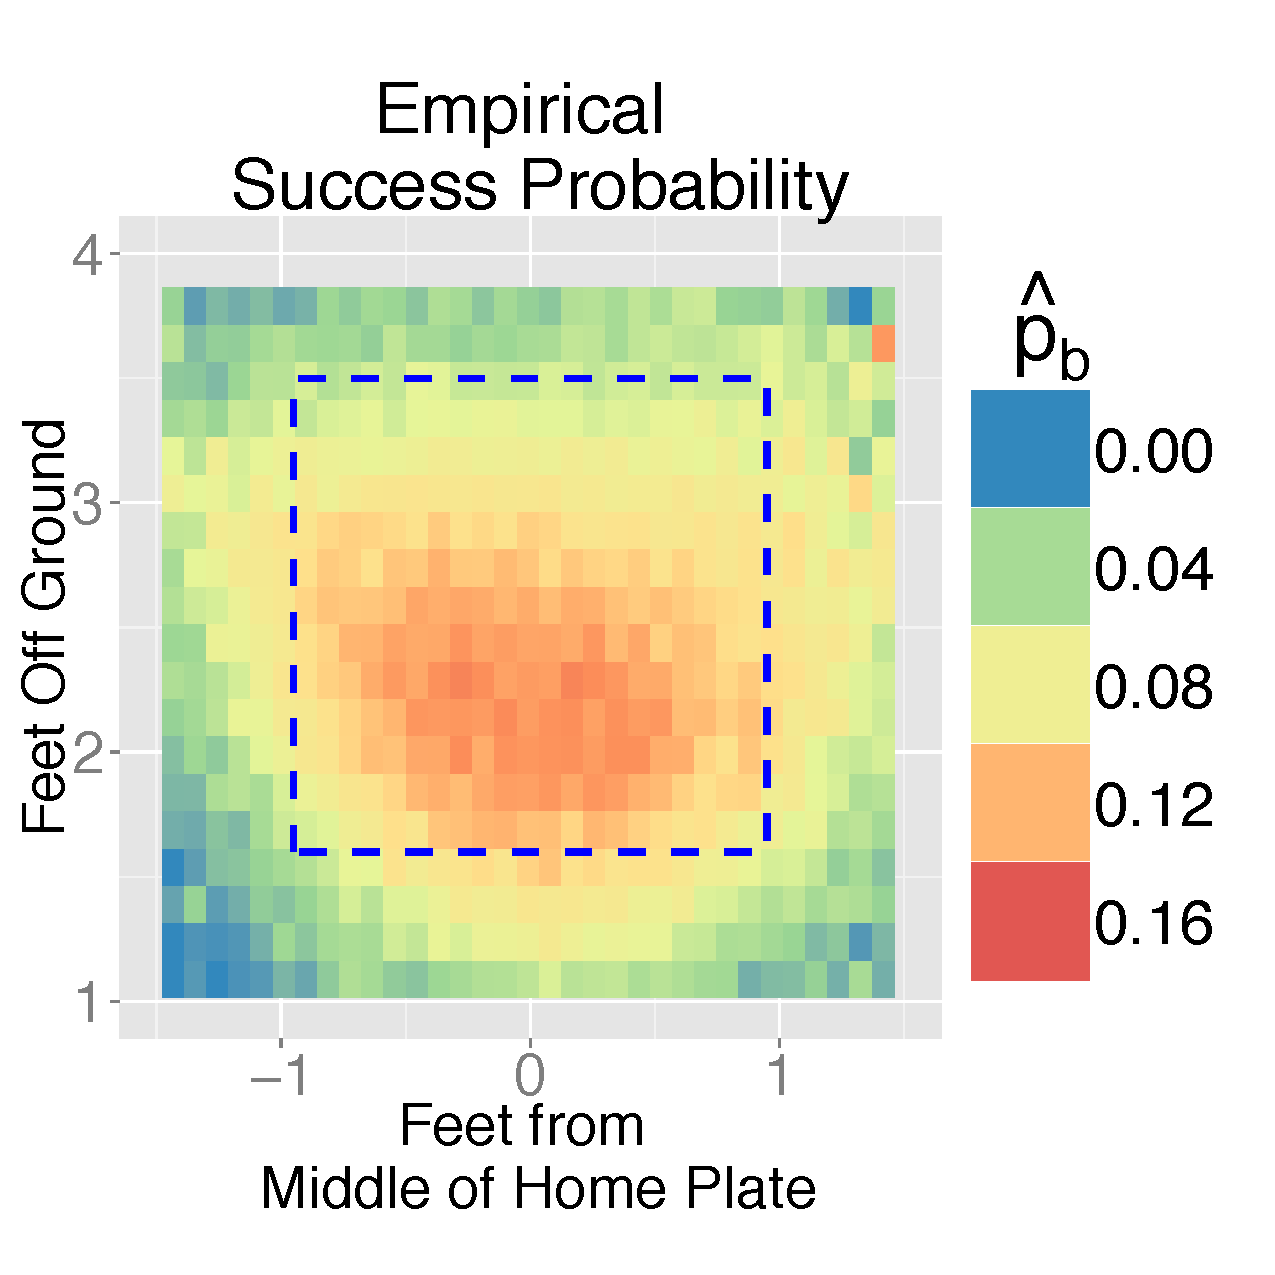
\includegraphics[scale=.3]{Images/Mothership.pdf} 
  \caption{The gridded hitting zone with 3/4 inch by 3/4 inch boxes, from the catcher's point of view. The color of the box represents the empirical batting average ($\hat{p}_{b}$) for right handed hitters, swinging at pitches in that location. Calculations based on 1,932 right handed hitters, swinging at 1,582,581 pitches between 2008 and 2015. The dashed line marks the boundaries of the called strike zone for a 6'2'' hitter.}
	\end{figure} 
	
\noindent While not sophisticated statistically, the graphic efficiently conveys empirical spatial success probabilities; it maps the statistic $\hat{p}_{b}$ to a color on a spectrum. Though it can easily go unnoticed, a heat map's creater {\it chooses} the grid box size that, hopefully, best communicates the data's information content; here, average spatial hitting ability estimates. The data's varying spatial density through the strike zone is not part of the communicated information, no matter the grid box size selected. This missing information is important, because in general more data means better estimates, and the viewer gets no such indication in Figure 1. Traditional heat maps do not communicate this information. We propose an innovation that addresses this shortcoming. To illustrate, consider a heat map for an individual hitter.

The heat map above divided the strike zone into relatively small boxes, because the data supported it. By ``supported it'' we mean the small, spatially specific boxes retain a sample size large enough to keep the variance of $\hat{p}_{b}$ acceptably \footnote{Defining ``acceptable'' variance ranges and thresholds will depend on context and analysis objectives. For example, a pitching coach may be satisfied with estimates accurate 95\% of the time to within 20 batting average points. This margin of error, 0.02, requires a sample size of 32 when $p_{b} = 0.09$. Note that the variance depends on the mean for a Bernoulli random variable.} This is important because individual hitter datasets vary dramatically in size, with swing totals ranging from a single swing to over 10,000 swings. Similar to bin width selection for a histogram, the choice of heat map resolution can dramatically affect how the data is represented, and the usefulness of the parameter estimates of interest. The resolution decision depends on the size and nature of the data set in question, and its spatial dispersion through the domain. To explore this decision in detail, we look at a heatmap for one batter.

\subsection{Resolution Selection} % ====== ======== ====== =======

Batter 425509, a veteran player named Jhonny Peralta, took 9,177 swings in this dataset. Peralta's swing data yields the heat map in Figure 2, which divides the central region of the strike zone into 16 equally sized boxes. Each box maps $\hat{p}_{b}$ to a color, and the box sample size, $n_{b}$, is printed on the box center. For convenient referencing in this chapter, we adopt the convention of numbering boxes with a horizontal component (left to right) and a vertical component (bottom to top [ {\bf Alix: ``WHY?''}]). For example, we call the top-left box (1,4), and the bottom-right box (4,1). 
        \begin{figure}[H]
      	\centering
      	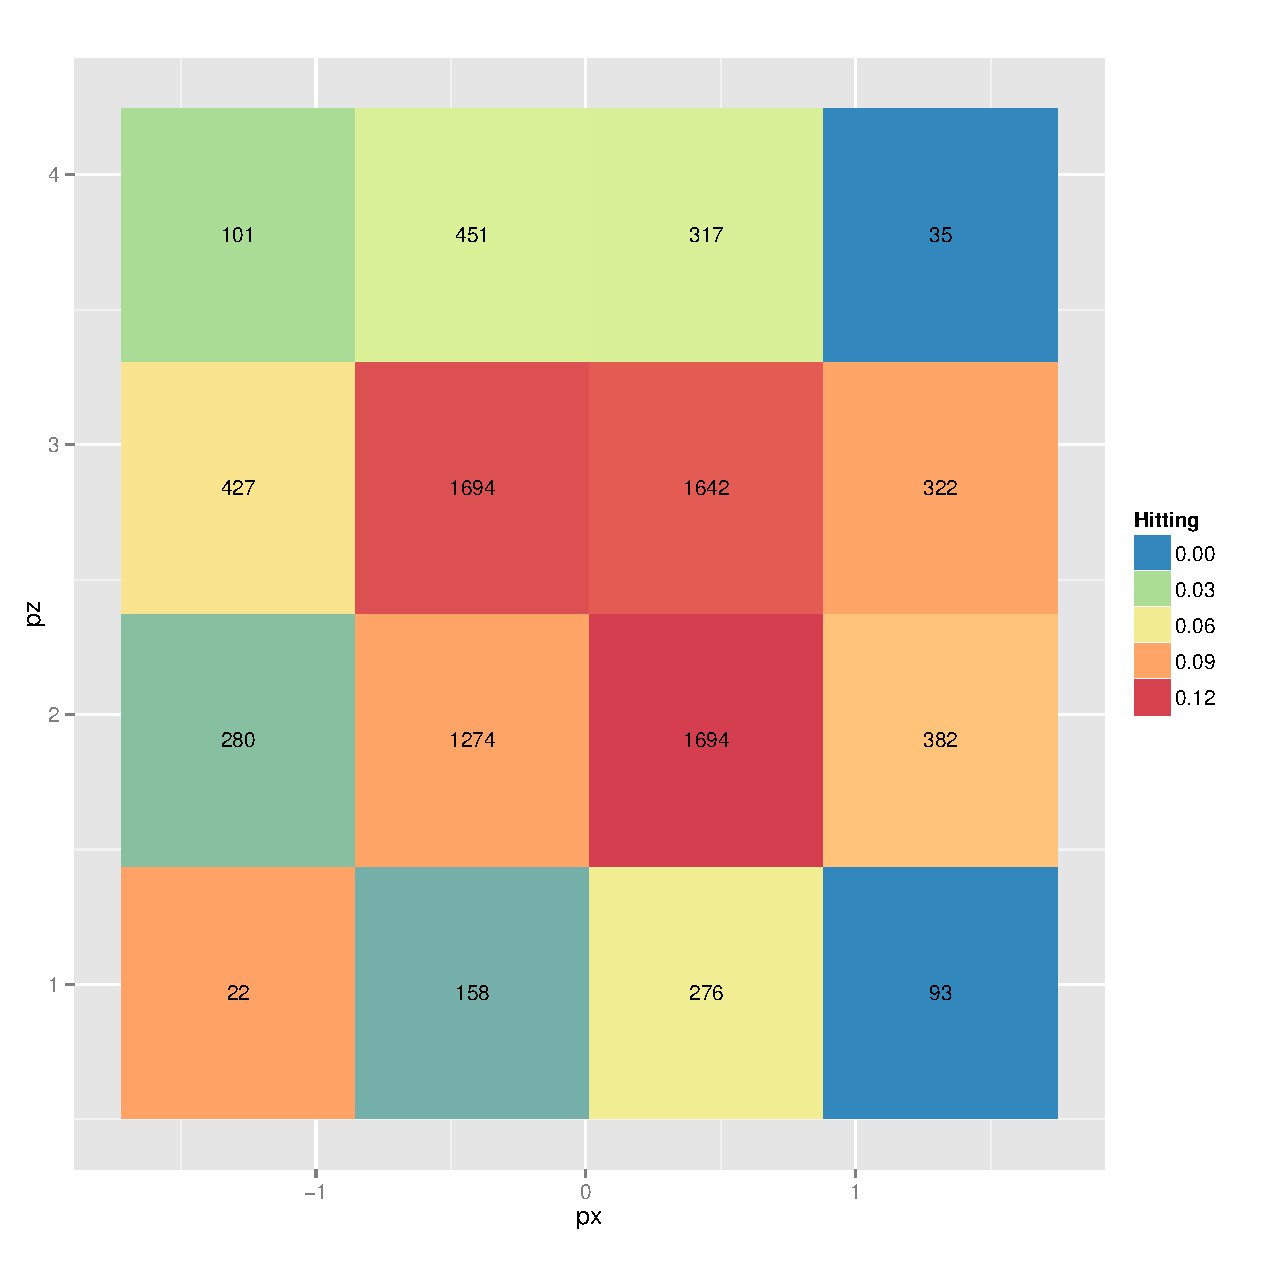
\includegraphics[scale=.35]{Images/Chapter4x4.pdf} 
      	\caption{This four by four heat map conveys the empirical batting average of batter 425509, Johnny Peralta, in each of 16 square regions of the hitting zone. Each box maps $\hat{p}_{b}$ to a color. The number printed on each box represents the number of pitches the hitter swung at that passed through that box.}
      	\end{figure} 

Peralta swang at 22 pitches in the region of space represented by box (1,1), and he swung at 1694 pitches in box (2,3). We interpret these two box sample sizes to contextualize. Three primary factors influence pitch location: pitcher game theoretic strategy, pitch-swing location margin of error (distance by which a pitch misses its intended target), and the game state. Game theoretic strategy concerns the pitcher's knowledge of the hitter's strenths and weaknesses, and the hitter's reciprocal knowledge. Margin of error concerns the pitcher's usual outcome of not exactly hitting his target.\footnote{If you visualize a 12 inch diameter archery target where the pitcher aims, he will usually hit the target somewhere, but not the bull's-eye.} Game state characteristics include the at-bat count, the number of outs, and if runners occupy bases.\footnote{Two example game state pressures include the increased penalty for throwing a pitch outside the strike zone on a three ball count (the runner gets on base at four balls); the increased penalty for a hit with a runner in scoring position (runner on second or third base).} Peralta probably swung at only 22 pitches in box (1,1) because he did not see many pitches there. We can speculate this is because pitches there are mostly out of the strike zone, both in the horizontal and vertical directions. Therefore, it is less likely to induce a swing at a bad pitch to hit, and unlikely to be called a strike despite being out of the strike zone. With $n_{(1,1)}=22$, the four by four resolution is sufficiently fine to present $\hat{p}_{(1,1)}$. Box (2,3), with $n_{(2,3)} = 1694$ pitches, can support more location specific, but still reliable estimates of $p$. This motivates finer resolution in that region of space. Peralta has relatively high success in Box (2,3), and he undoubtedly swings at as many pitches in that box as possible. The pitcher knows this, so will seldom aim there. However, by virtue of being closer to the center of the strike zone, this location collects more pitch location mistakes.

Because, as mentioned, a finer resolution is justified for box (2,3), we subdivide all boxes further. For simplicity, without implying this is the only or best way to increase resolution, we divide each box into four equally sized sub-boxes. Figure 3 shows the 16 by 16 result.
        \begin{figure}[H]
      	\centering
      	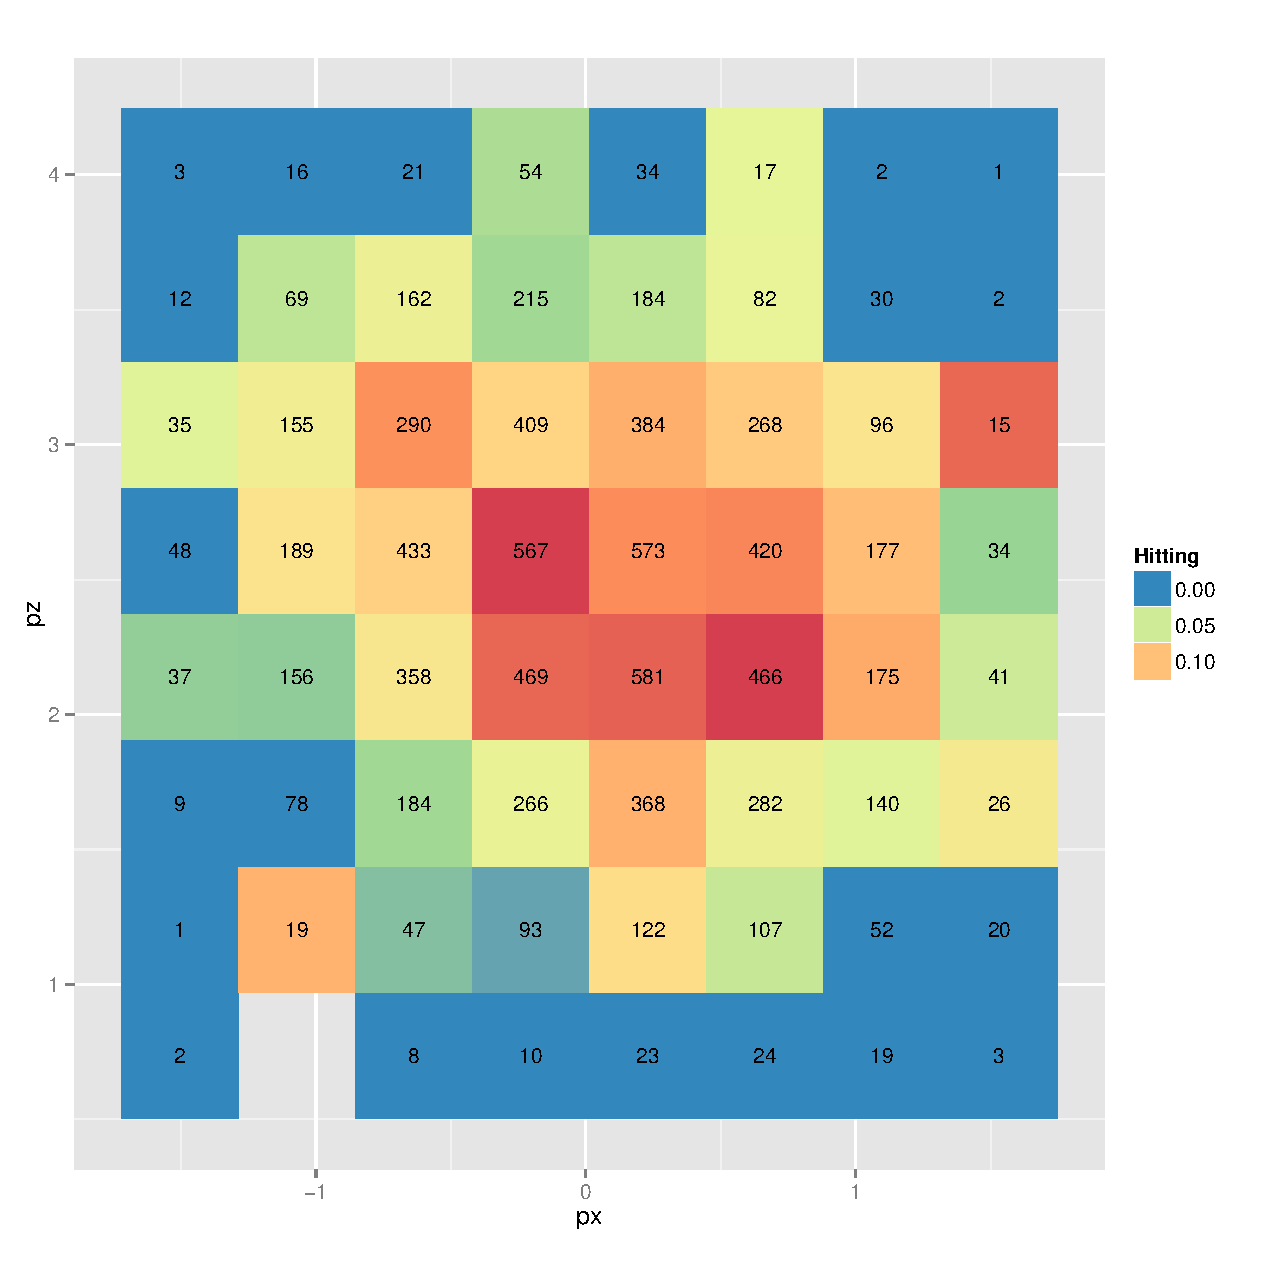
\includegraphics[scale=.25]{Images/Chapter16x16.pdf} 
      	\caption{This 16 by 16 heat map conveys the empirical batting average of batter 425509, Johnny Peralta, in each of 64 square regions of the hitting zone. Each box maps $\hat{p}_{b}$ to a color. The number printed on each box gives the number of pitches the hitter swung at that passed through that box. A grey box indicates no pitches passed through that box.}
      	\end{figure} 

Boxes (3,5), (3,6), (4,5), and (4,6)---the boxes created by dividing box (2,3) at the four by four resolution---still contain sample sizes sufficient to support low variance $p$ estimates. More generally, 24 boxes still have a sample size greater than 150; and 15 boxes still have a sample size of greater than 250. These boxes could support further subdivision. On the other hand, numerous boxes---corner and edge boxes in particular---now contain sample sizes generally insufficient to support low variance estimates of $p_{b}$. Twenty-nine boxes have a sample size of less than 50, and 17 boxes have a sample size of less than 20. At this resolution one box recorded zero swings.

In this way, due to the particular dispersion of the data, a heat map at any resolution will contain boxes of exceedingly small sample sizes (high variance), and/or boxes of unnecessarily large sample size (unnecessarily low variance). Figure 3 shows six different heat map resolutions, constructed with the same data from Peralta. We started with one box, and subdivided each box into four at each iteration. We chose this simple resolution increasing algorithm to illustrate the resolution selection challenge, and to provide a foundation for our innovation in the next section. 
        \begin{figure}[H]
      	\centering
      	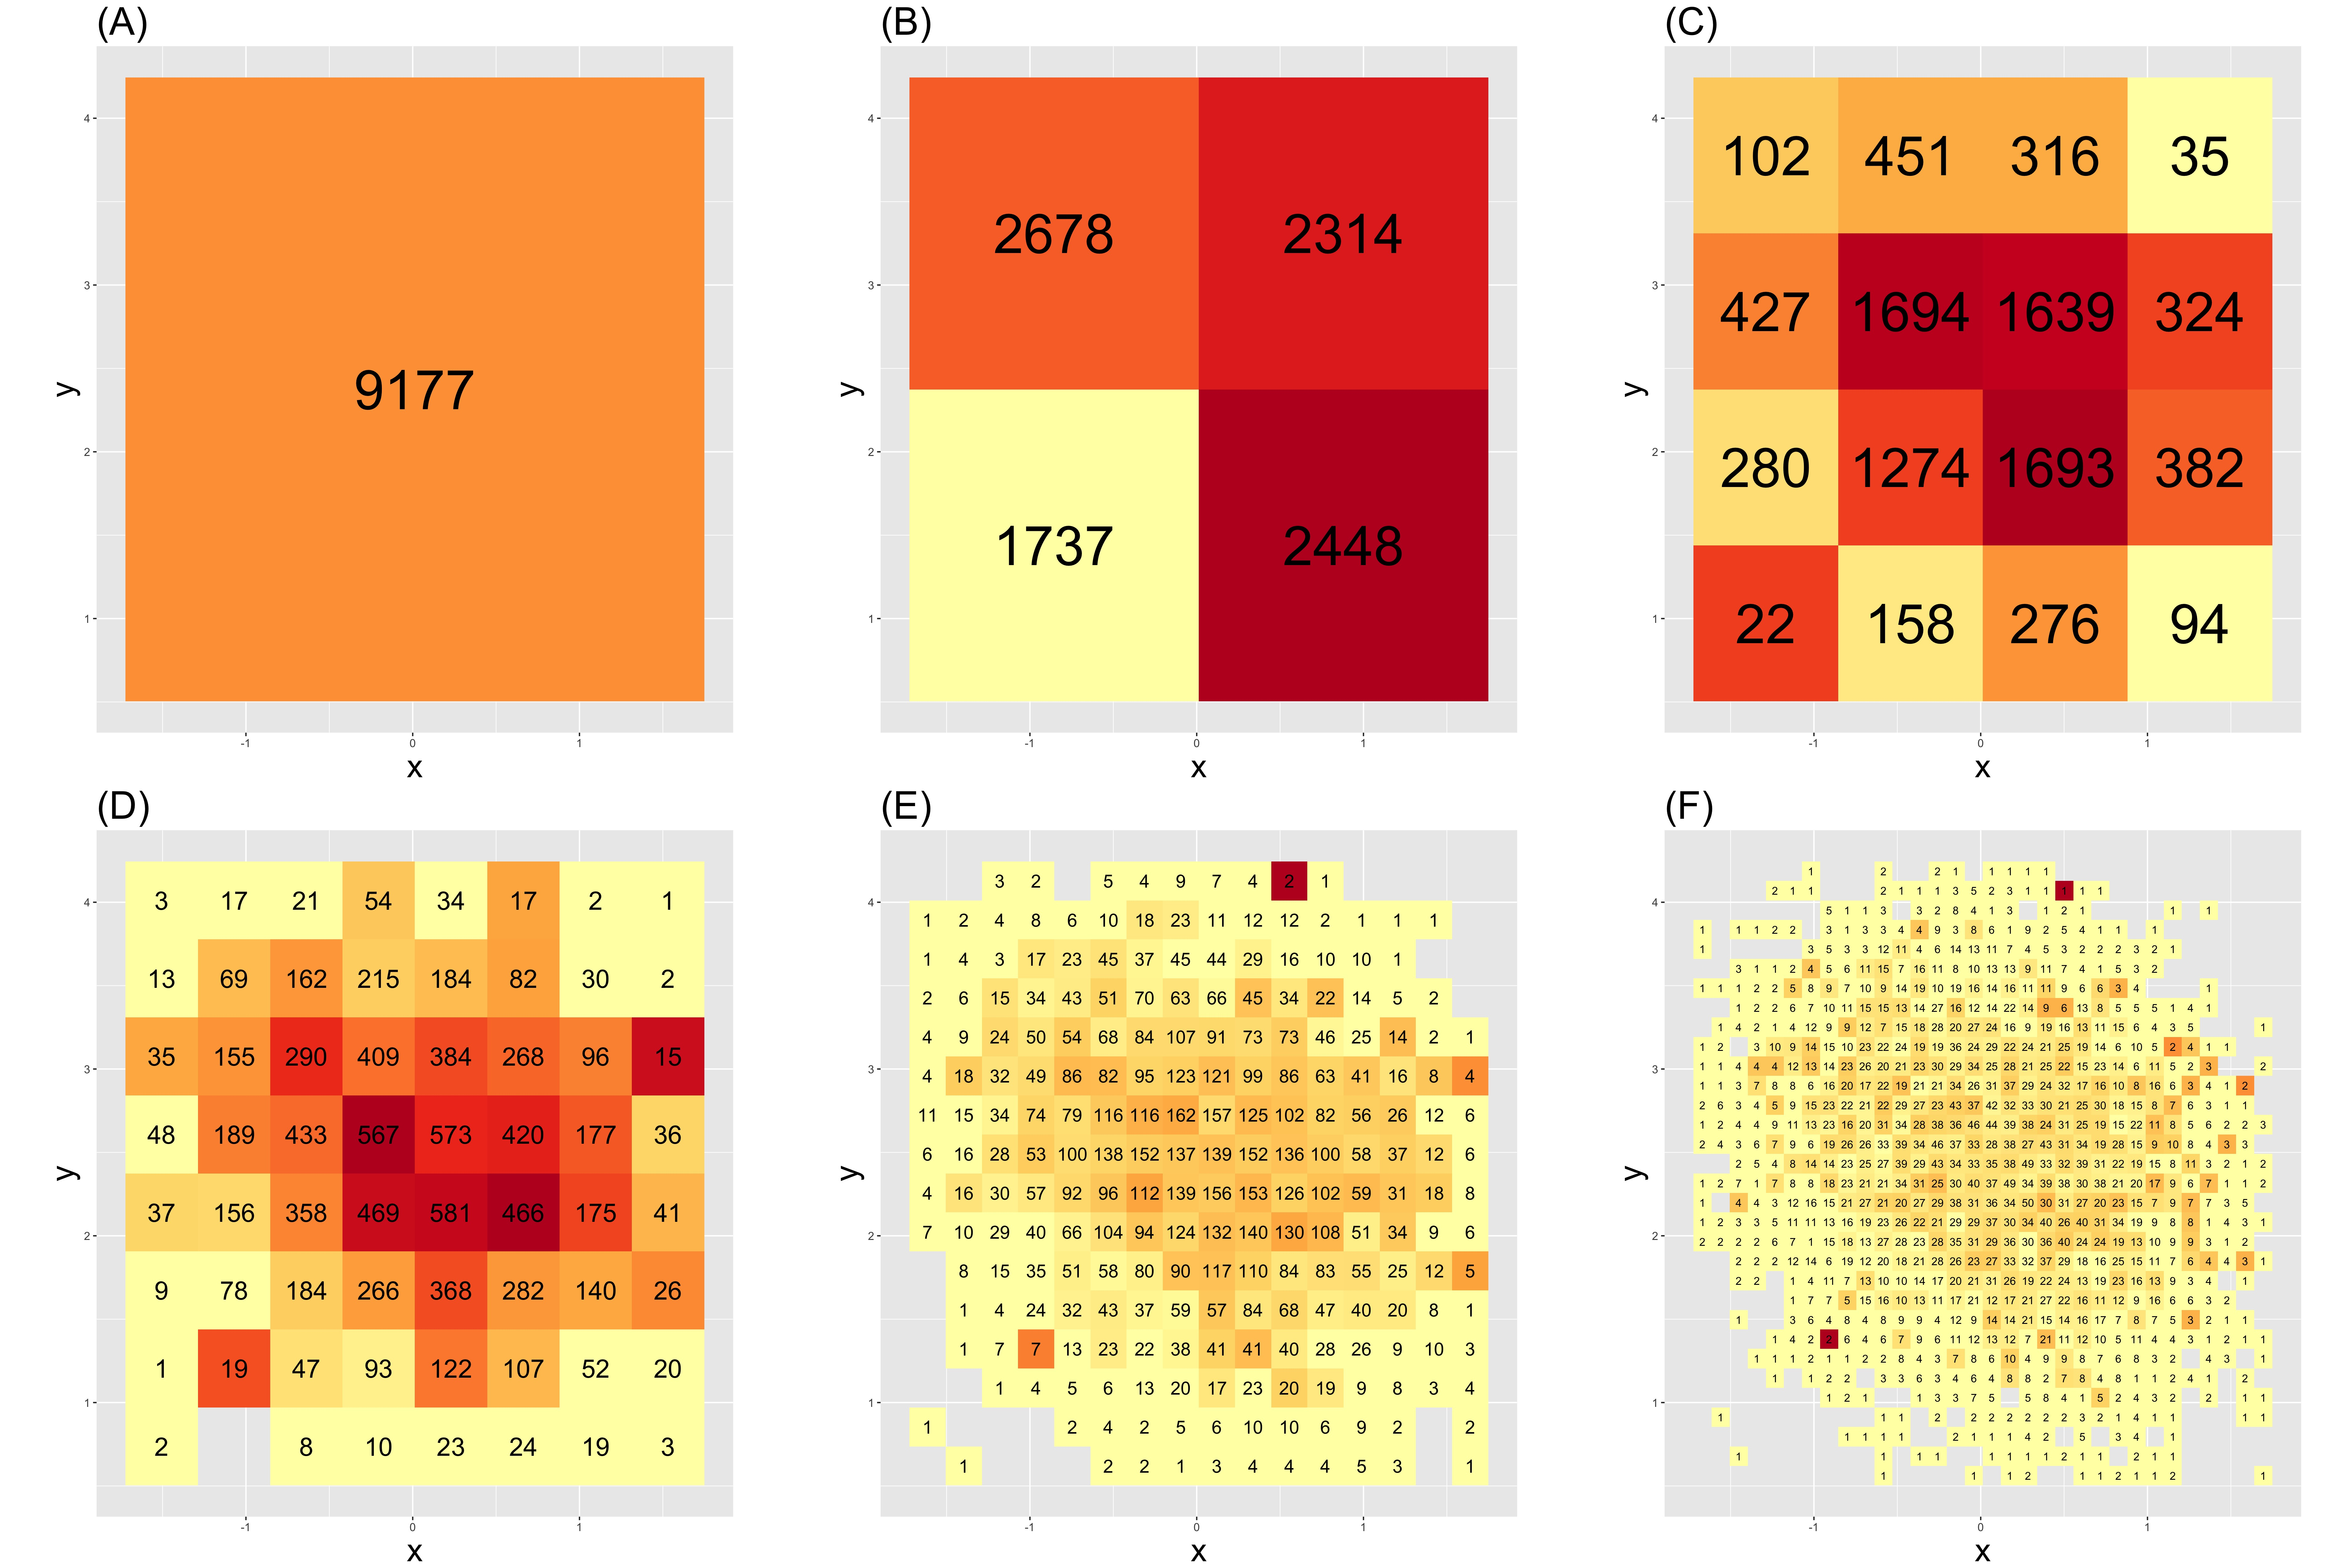
\includegraphics[scale=.4]{Images/Chapter_VarRes.png} 
      	\caption{These {\bf six (?)} heat maps show the same data, 9177 swings by batter 425509, Johnny Peralta, at increasing resolutions. Heat map one is unnecessarily coarse, while heat map six is excessively fine. Note how dramatically the visual imact and impression varies as the resolution increases. Which resolution best conveys the data?}
      	\end{figure} 

It is unclear which of these five resolutions best combines spatially precise estimates of $p$ where possible, and box sample sizes with $\text{Var}(\hat{p}_{b})$ in a desirable range. The viewer interested in the center of the strike zone should prefer the last ({\bf need labels} heat map, as the box sample sizes are sufficient to provide such spatially specific low variance estimates. The boxes closer to the edges of the strike zone contain higher variance, and thus less reliable estimates, due to prohibitively small sample sizes. We propose a new heat map approach that combines resolutions according to the data's varying spatial density.

\subsection{Empirical Heat Maps and Spatially Varying Resolution} % ==========

Consider again the heat map in Figure 2. Notice box (1,1) contains data on 22 swings, a sample size where subdividing would yield sample sizes uselessly small, and thus estimate variances prohibitively high. Box (2,3), in contrast, contains data on 1694 swings, which would support estimates that are more spatially accurate without $\text{Var}(\hat{p}_{b})$ increasing past acceptable levels. We propose defining a stopping rule and a subdividing method, and subdividing boxes further accordingly. For example, in Figure 4 we subdivide, into four equally sized boxes, all boxes where $n_{b} > 200$, . One iteration through all boxes at their current size, subdividing according to this rule, converts the heat map on the left to the heat map on the right.
        \begin{figure}[H]
      	\centering
      	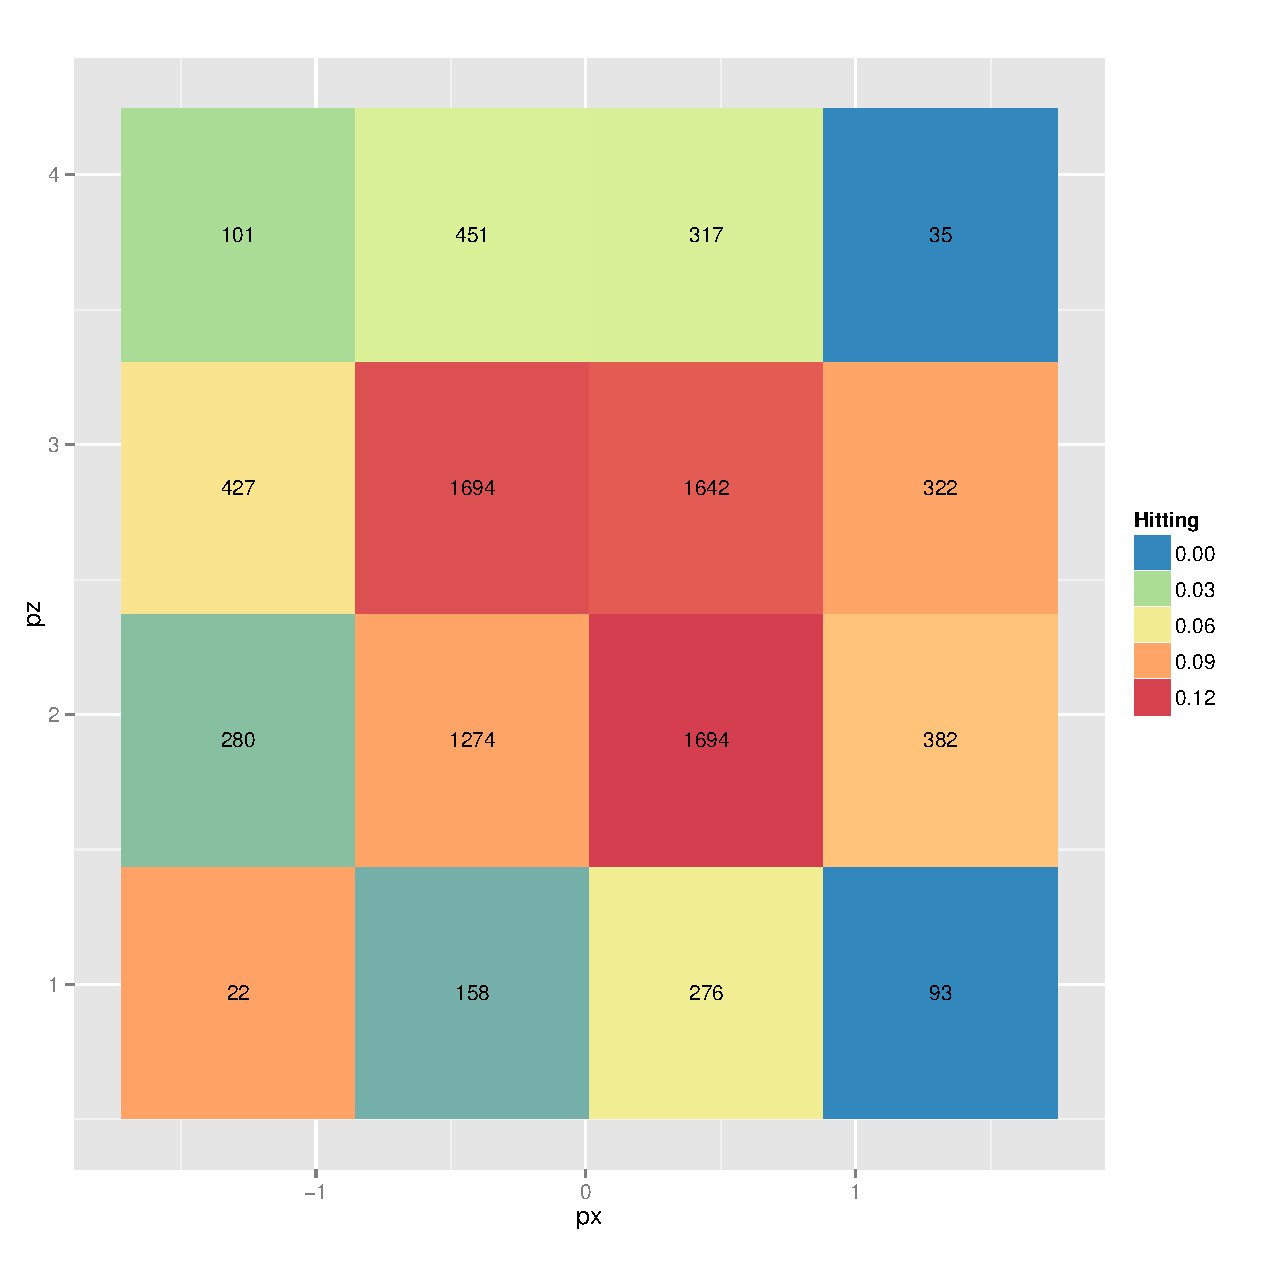
\includegraphics[scale=.3]{Images/Chapter4x4.pdf} 
      	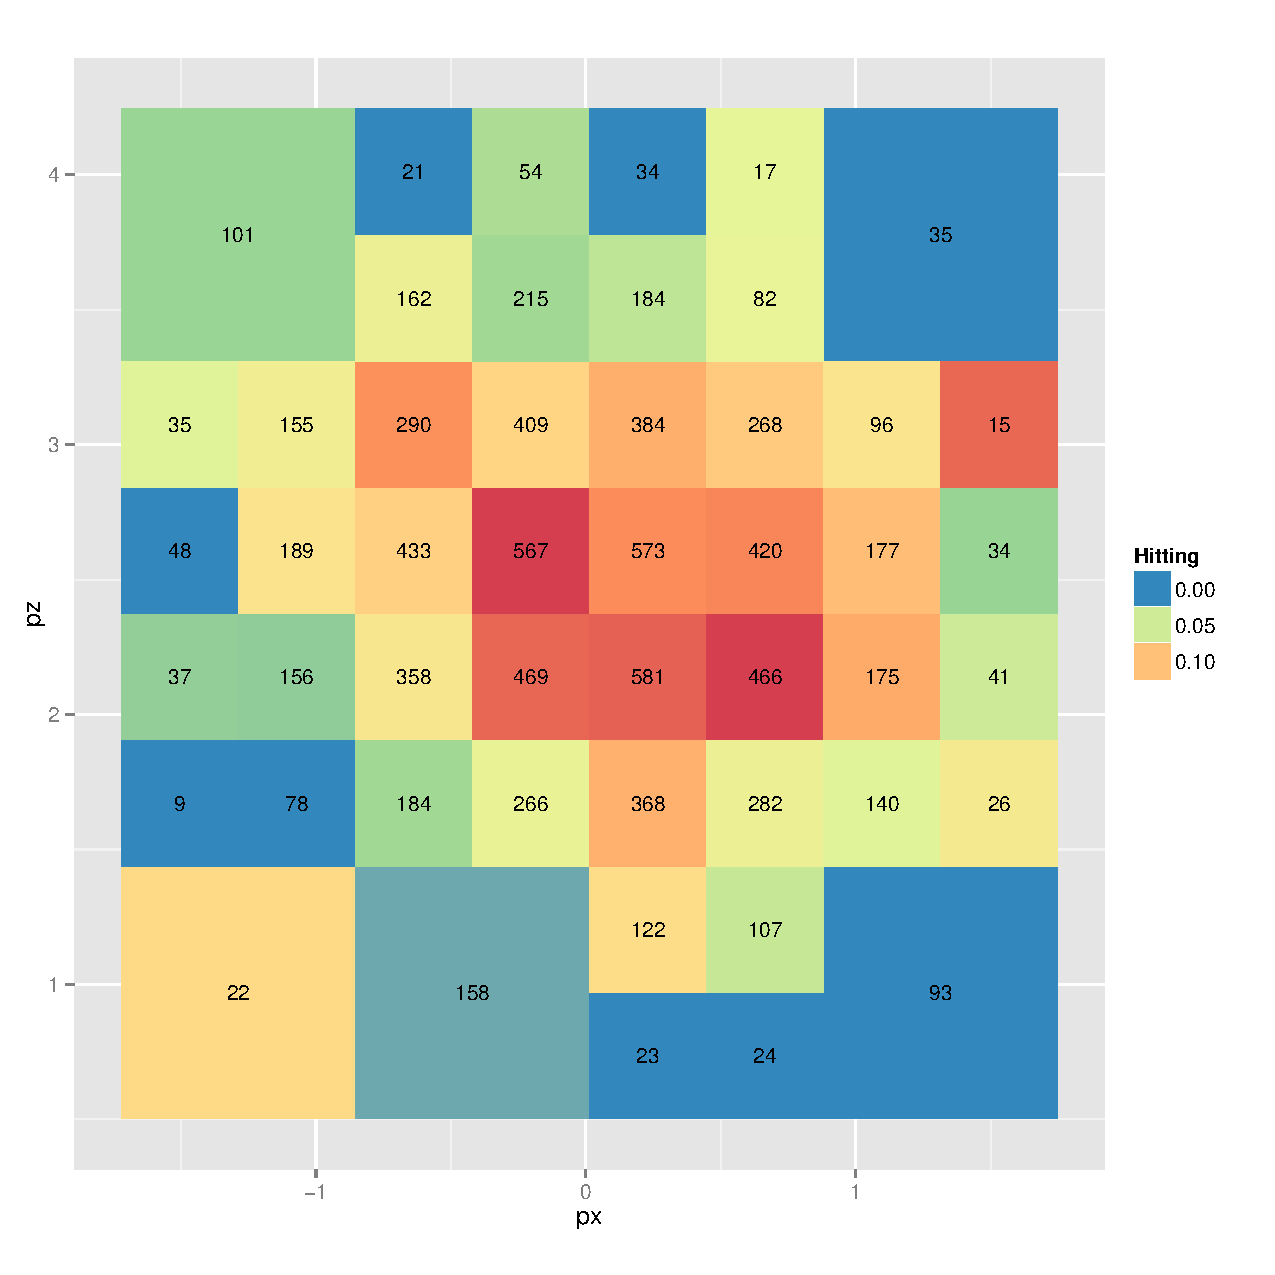
\includegraphics[scale=.3]{Images/Chapter8x8_200.pdf} 
      	\caption{These heat maps convey the empirical batting average of Johnny Peralta in each square region of the hitting zone. Each box maps $\hat{p}_{b}$ to a color. The number printed on each box represents the number of pitches Peralta swung at that passed through that box. Notice that all boxes with a sample size greater than 200 in the heat map on the left, have been subdivided in the heat map on the right.}
      	\end{figure} 
Notice all four corner boxes have not subdivided, indicating Peralta seldom sees and swings at pitches in these locations. The boxes toward the middle of the map tend to have larger sample sizes, and higher $\hat{p}_{b}$. Pitches pass through the middle of the hitting zone more frequently because many pitch target margin of error circles overlap there; and it is the region where pitch target margin of error circles are entirely inside the strike zone. Sixteen boxes still have a sample size greater than 200, and 11 still have a sample size greater than 300. We iterate again, and further subdivide 16 boxes where $n_{b} > 200$.
        \begin{figure}[H]
      	\centering
      	
      	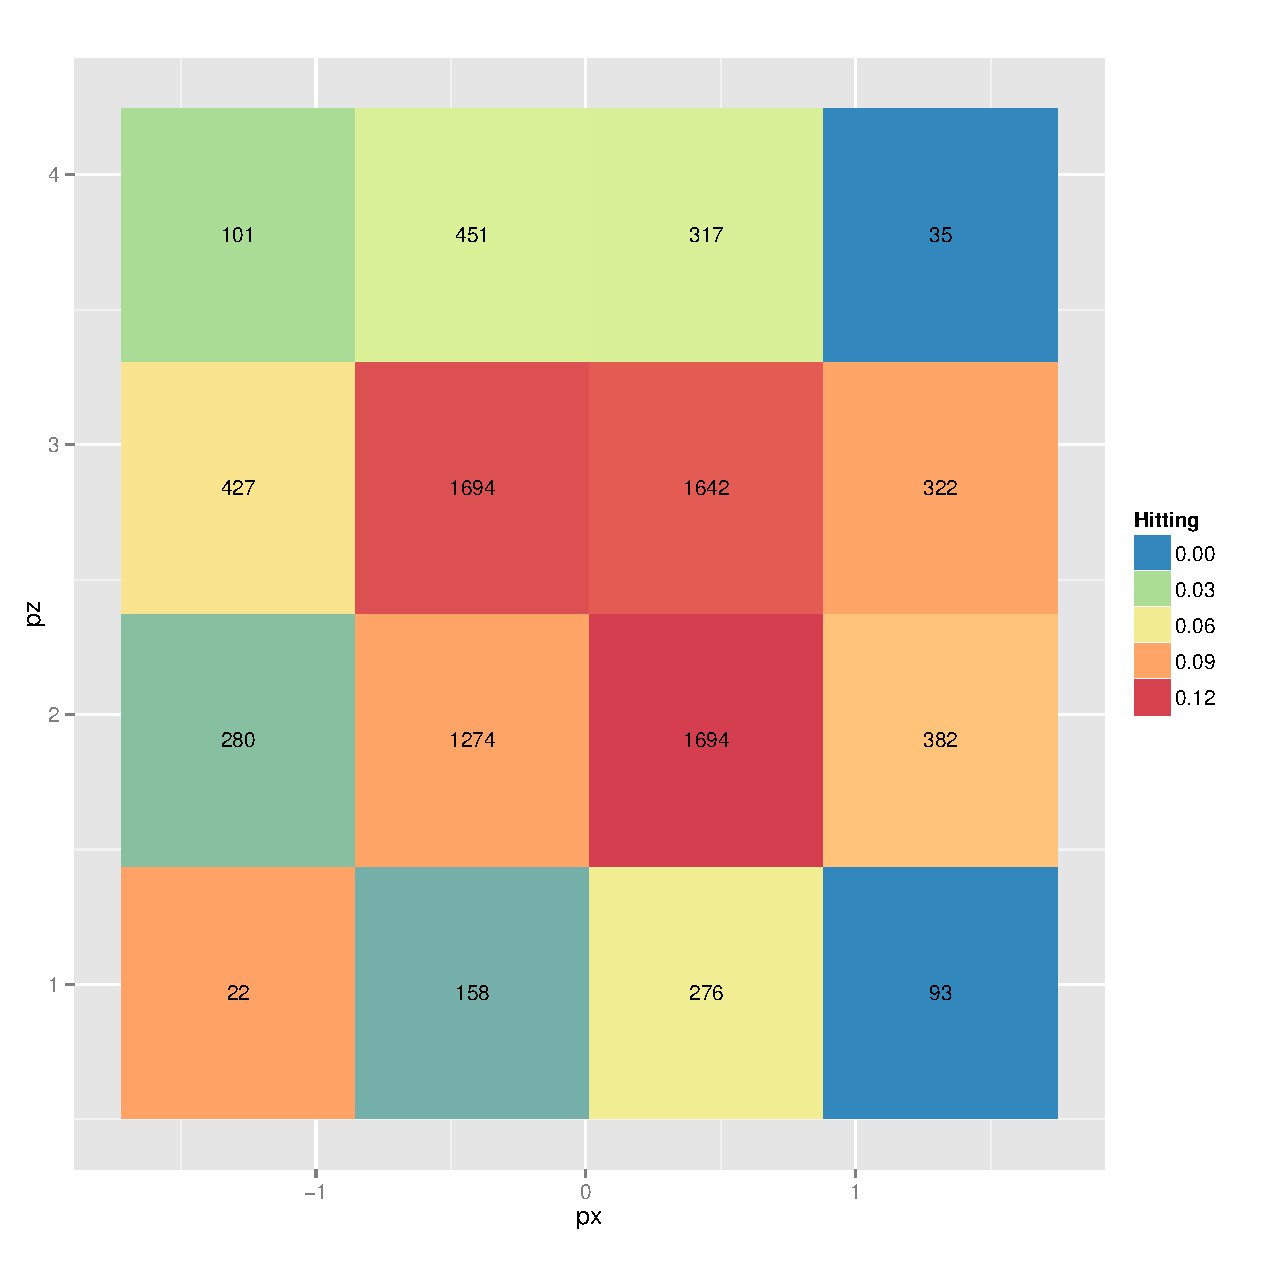
\includegraphics[scale=.25]{Images/Chapter4x4.pdf}
      	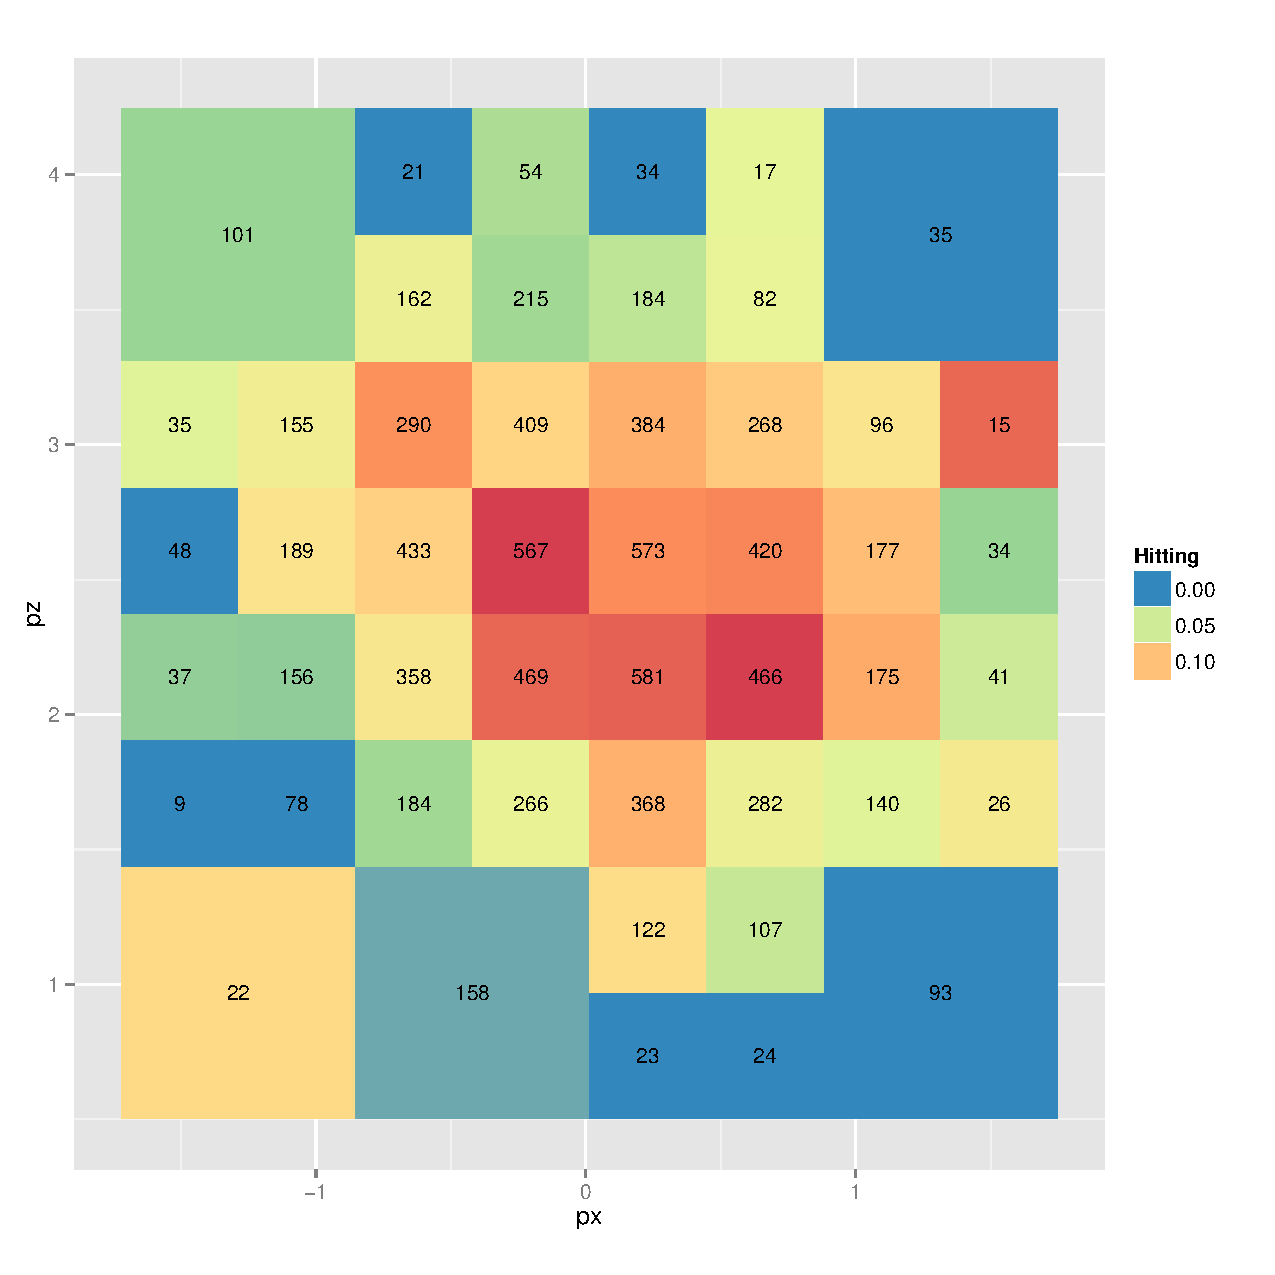
\includegraphics[scale=.25]{Images/Chapter8x8_200.pdf} 
      	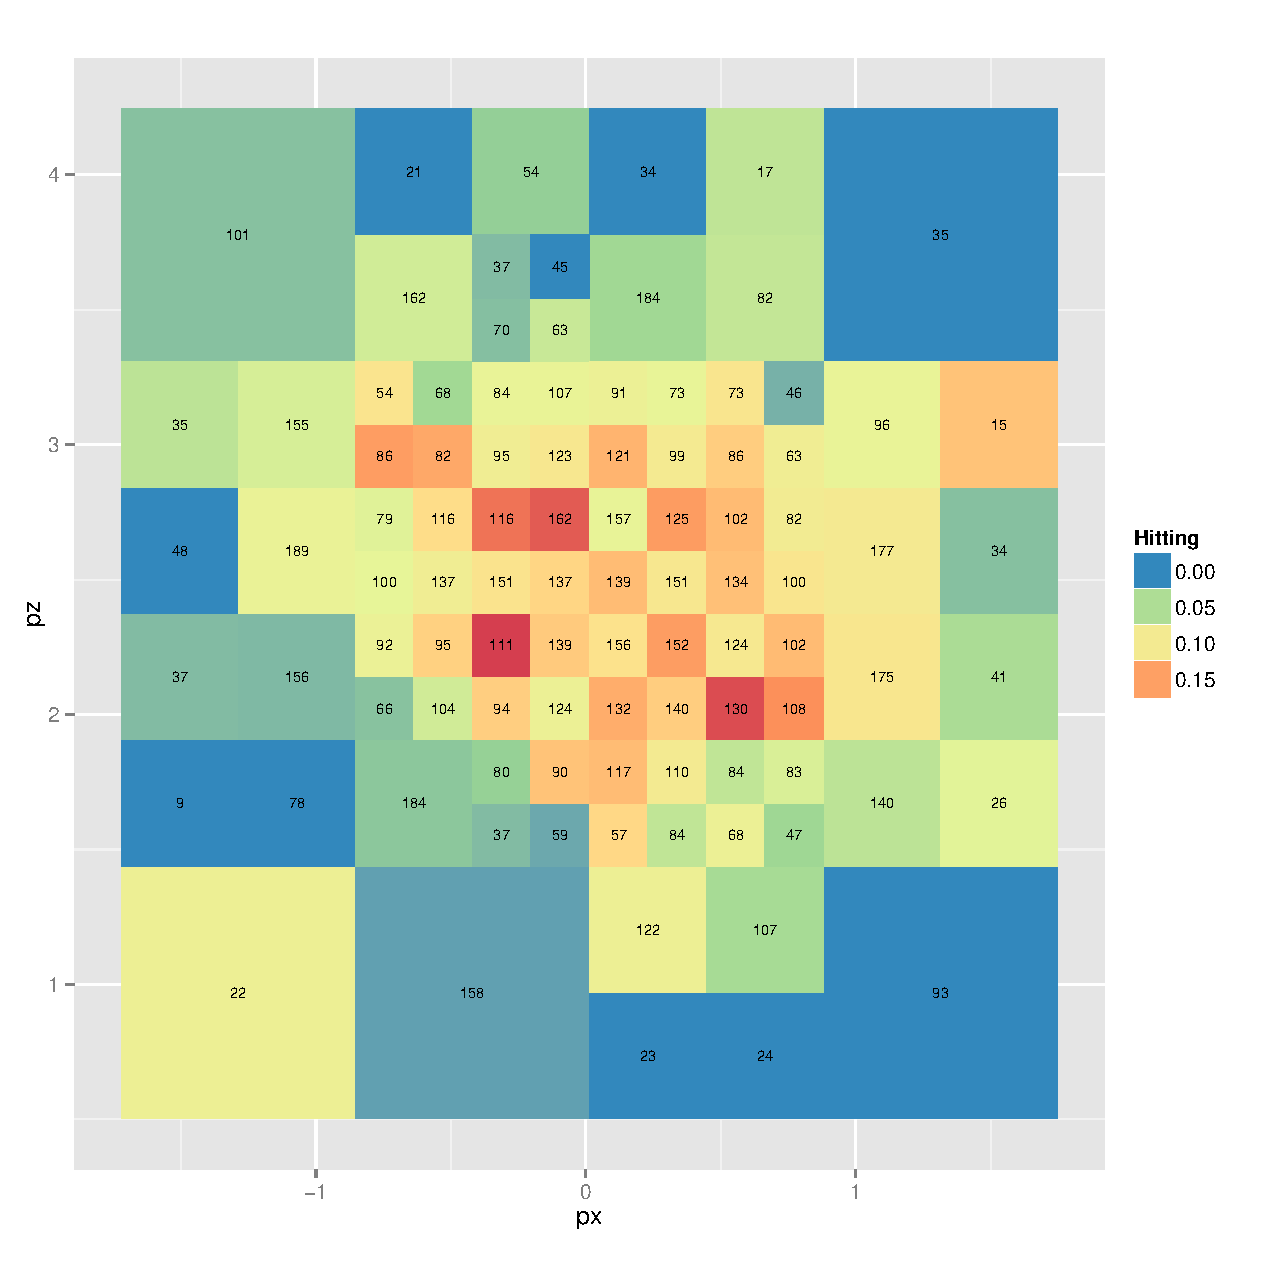
\includegraphics[scale=.25]{Images/Chapter16x16_200.pdf} 
      	\caption{These heat maps convey the empirical batting average of batter 425509, Johnny Peralta, in each boxed region of the hitting zone. Each box maps $\hat{p}_{b}$ to a color. The number printed on each box represents the number of pitches the hitter swung at that passed through that box. All boxes with a sample size greater than 200 in the heat map on the left, have been subdivided in the heat map in the middle. All boxes with a sample size greater than 200 in the heat map in the middle, have been subdivided in the heat map on the right.}
      	\end{figure}
In Figure 6, the middle heat map has 16 boxes with $n_{b} > 200$. In the heat map on the right these 16 boxes have been subdivided into four boxes each. After this iteration, the heat map on the far right consists of 97 boxes, with a mean box sample size of 94.57, and median of 94. The minimum box sample size is 9, and the maximum is 189. The first quartile box sample size is 63, and the third quartile is 125. Regions with a higher density of pitch-swings necessarily have smaller boxes, which acts to convey additional information to the reader, compared to a heat map on a uniform grid. Note that the stopping rule and subdivision algorithm can be defined by the map's creator, offering flexibility to create the heat map structure that suits the data. 

Figure 8 gives the full sequence of heat maps that result from applying the stopping rule $n_{b} < 100$, starting with a single box.
        \begin{figure}[H]
      	\centering
      	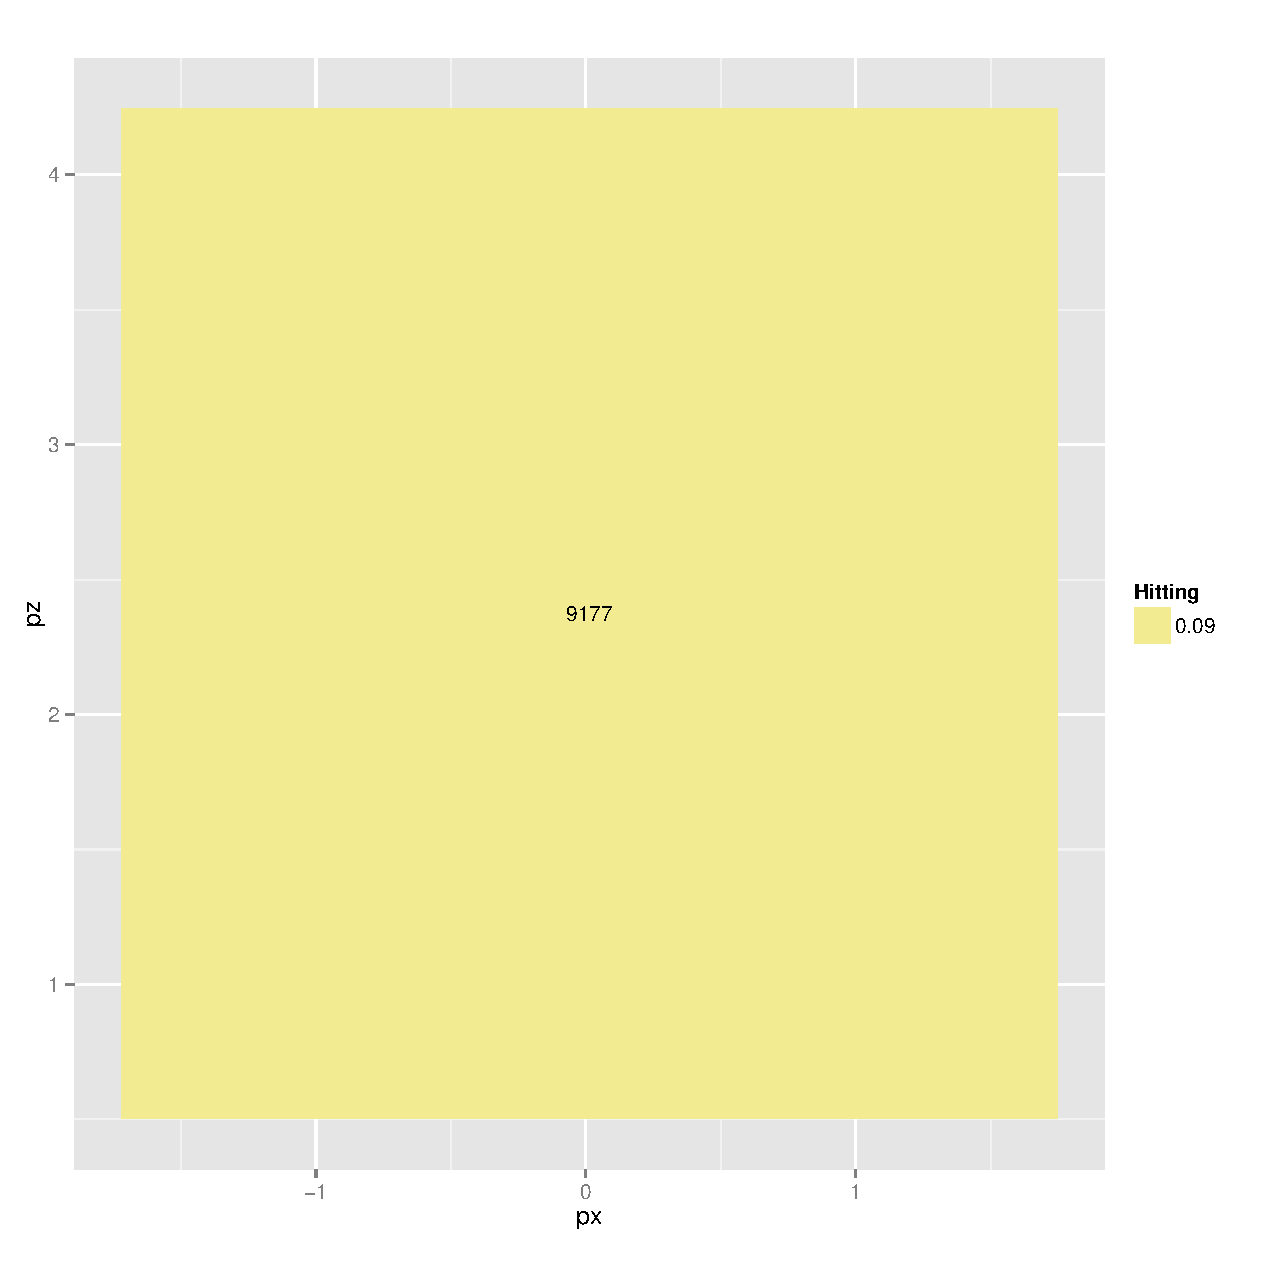
\includegraphics[scale=.2]{Images/Chapter1x1.pdf}
      	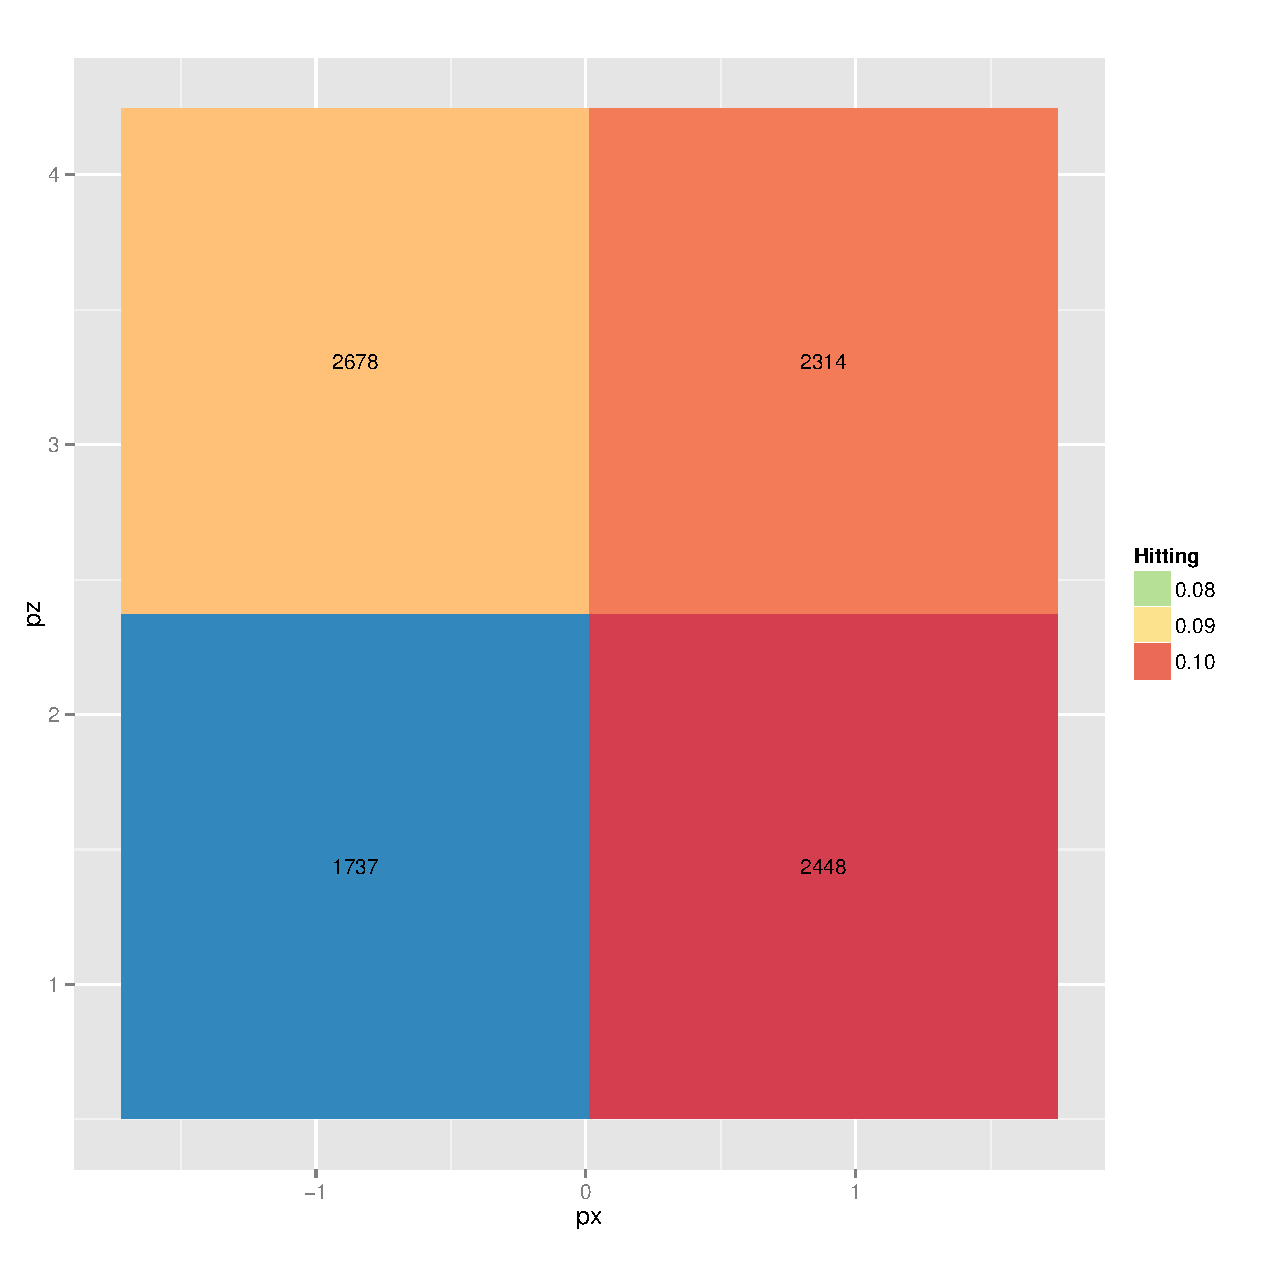
\includegraphics[scale=.2]{Images/Chapter2x2.pdf}
      	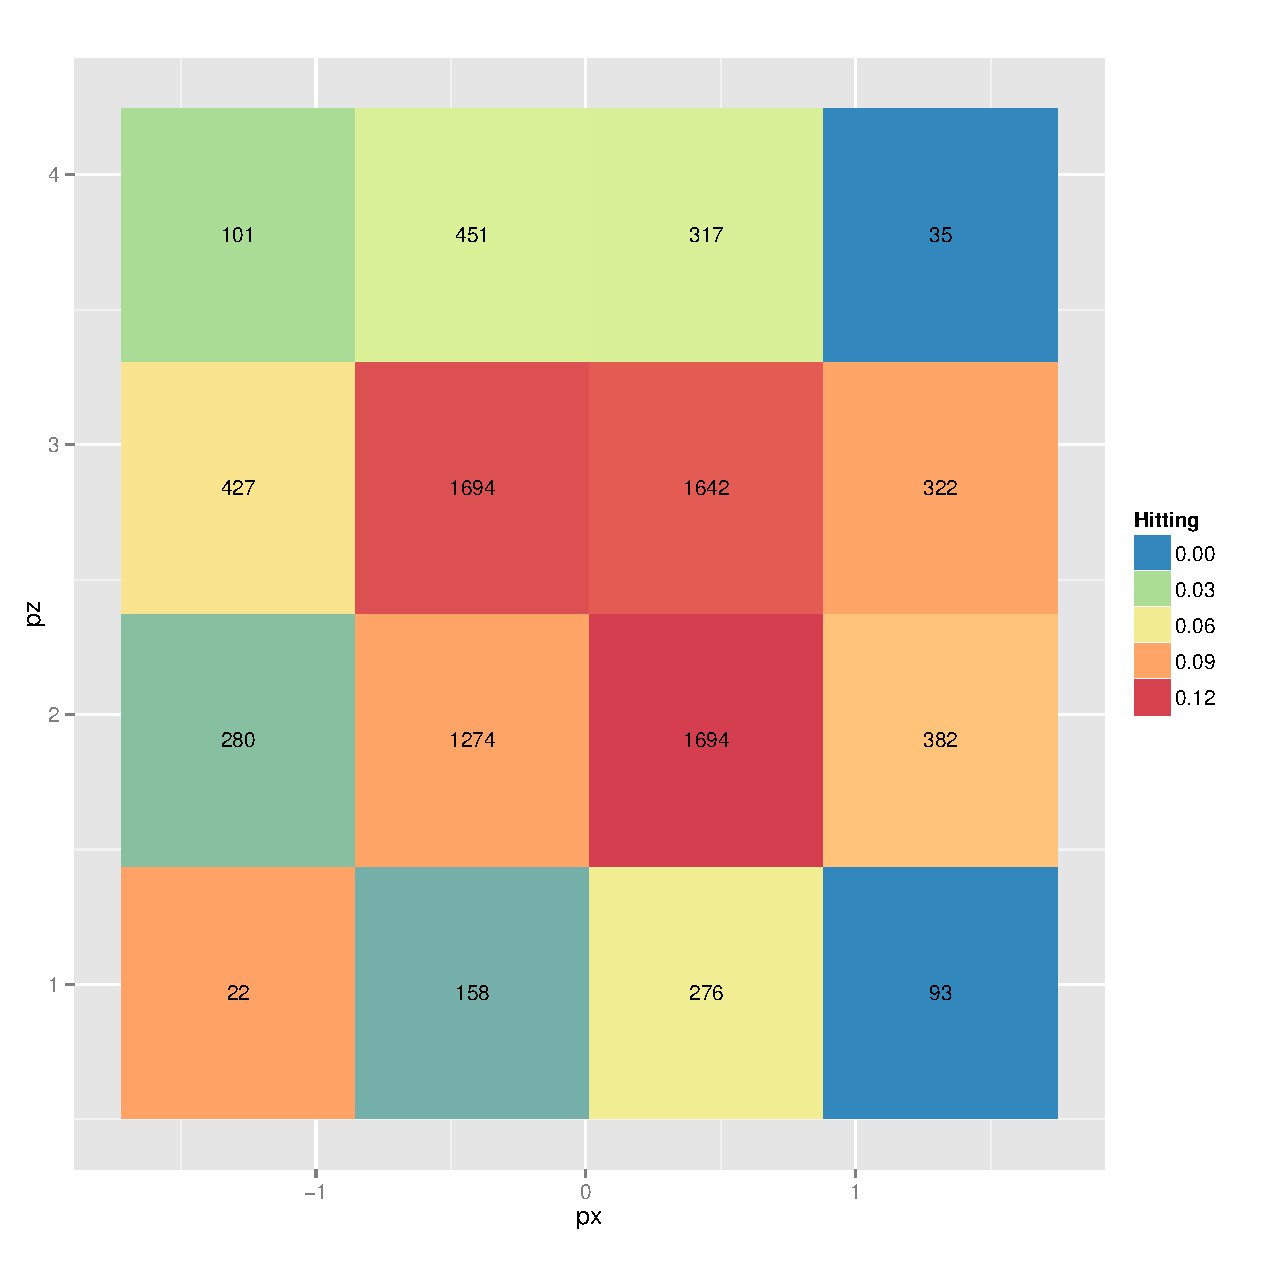
\includegraphics[scale=.2]{Images/Chapter4x4.pdf}
      	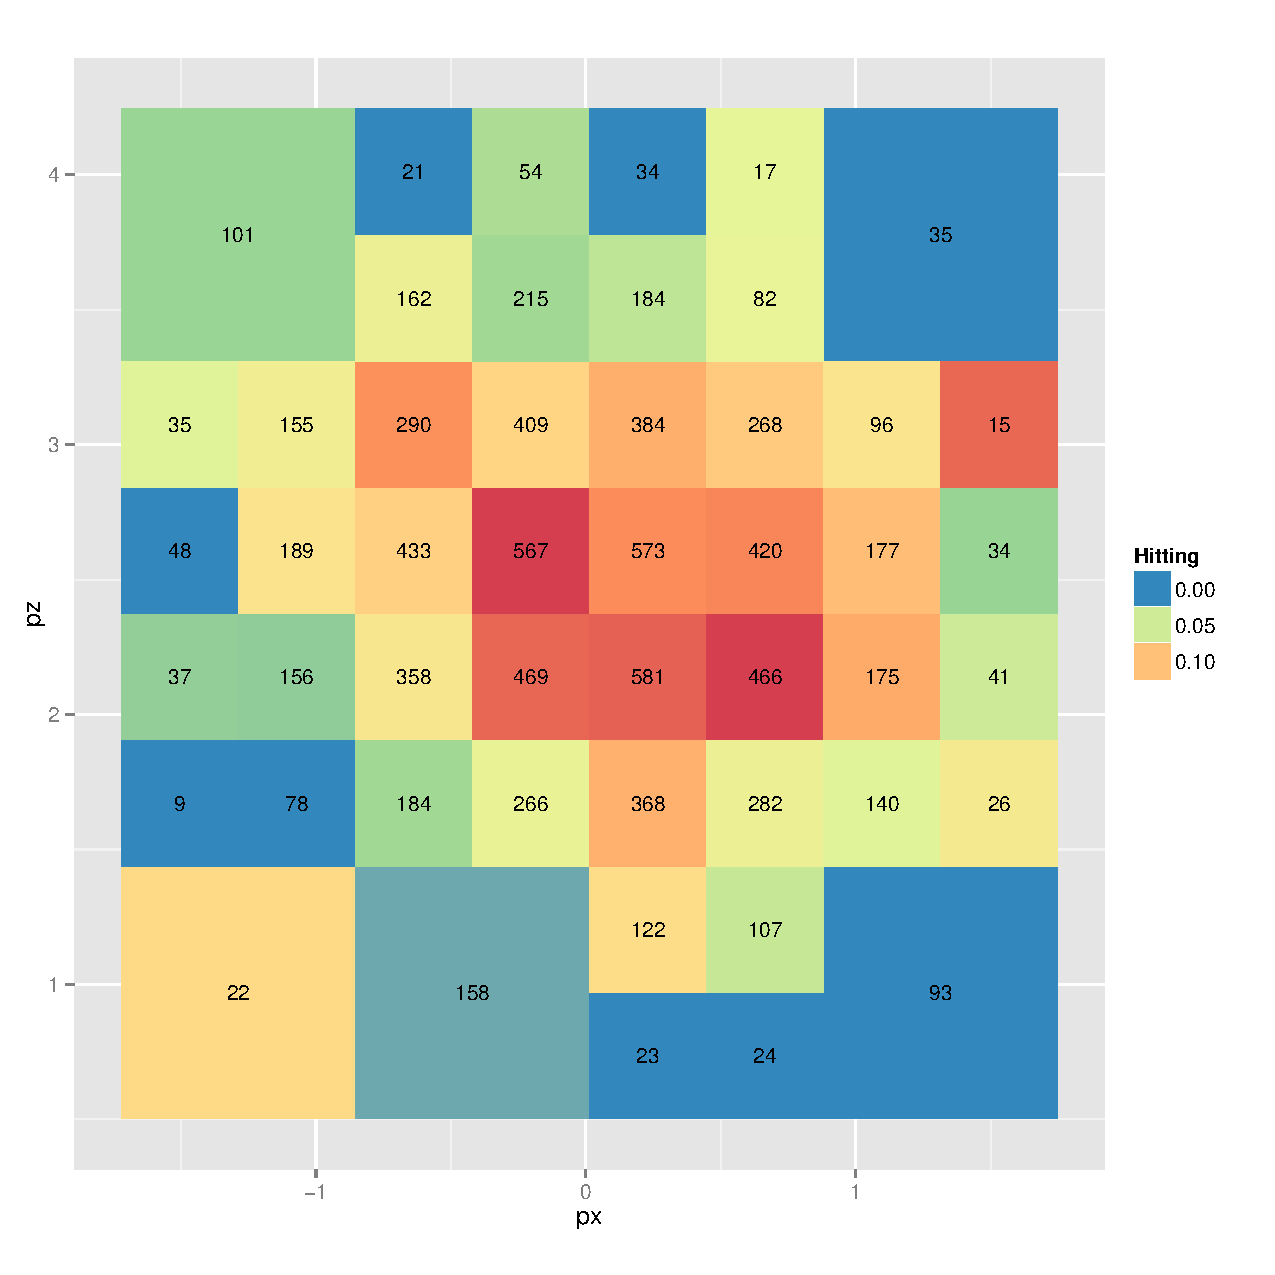
\includegraphics[scale=.2]{Images/Chapter8x8_200.pdf} 
      	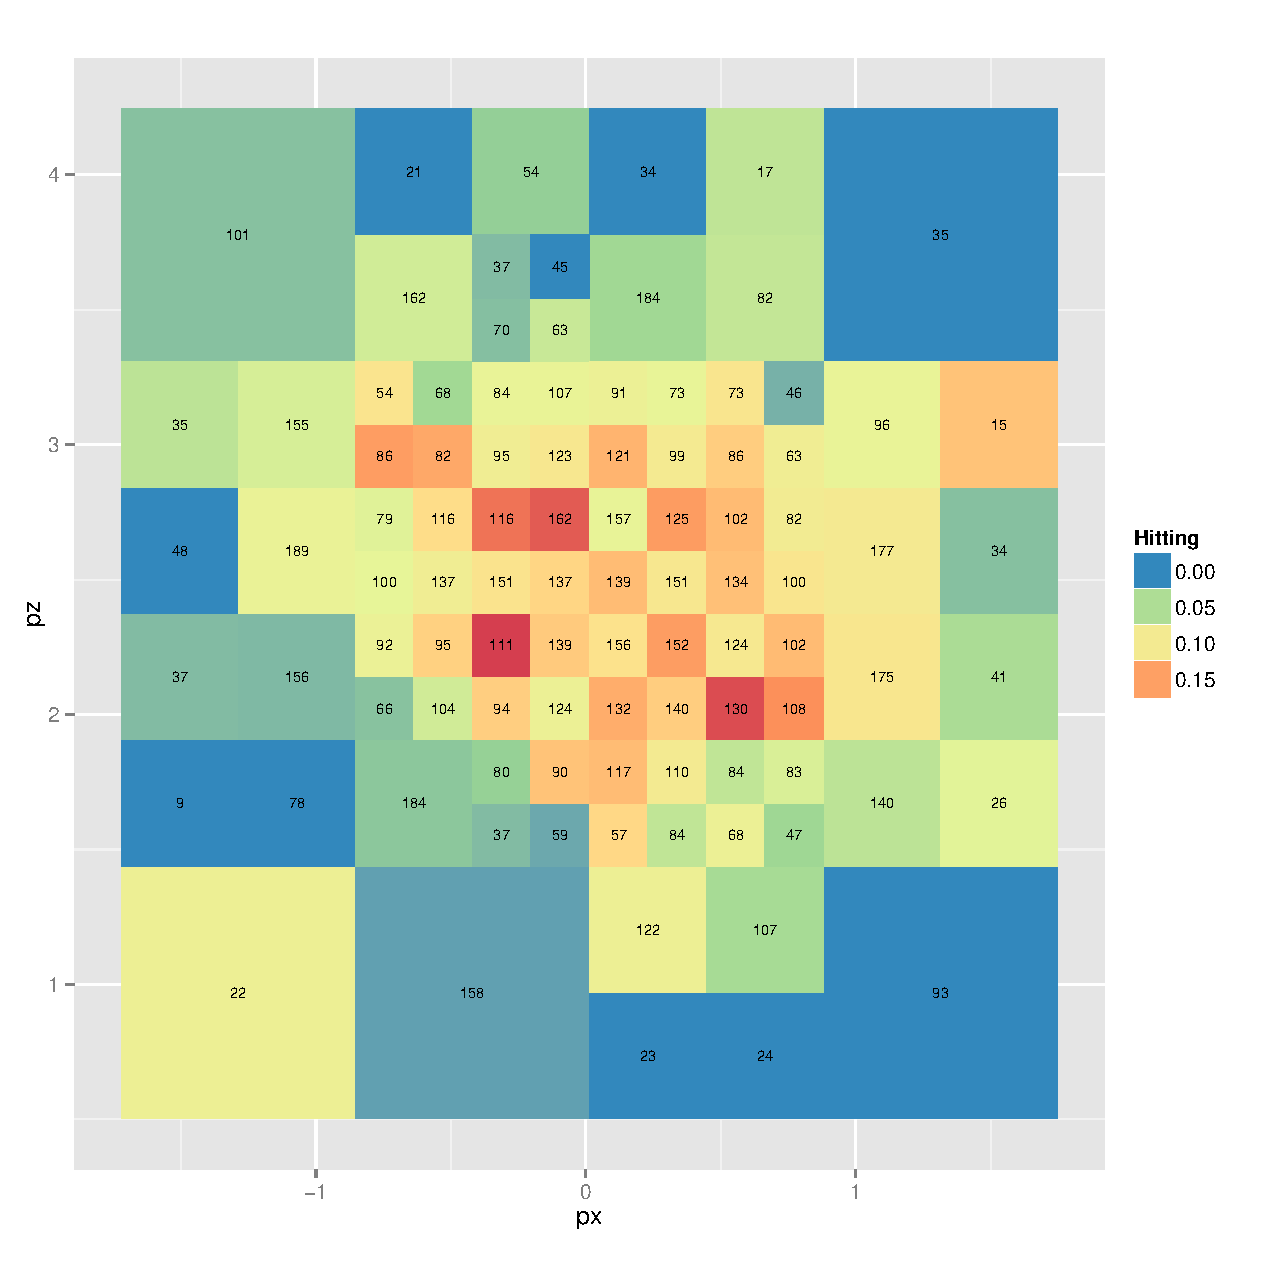
\includegraphics[scale=.2]{Images/Chapter16x16_200.pdf} 
      	\caption{These heat maps convey the empirical batting average of batter 425509, Johnny Peralta, in each boxed region of the hitting zone. Each box maps $\hat{p}_{b}$ to a color. The number printed on each box represents the number of pitches the hitter swung at that passed through that box. All boxes with a sample size greater than 200 in each heat map have been subdivided in the subsequent heat map.}
      	\end{figure}

To demonstrate the flexibility, consider a different stopping rule, $n_{b} < 100$. Figure 8 gives the sequence of heat maps that result from applying this stopping rule, with the same subdividing algorithm (***need to delineate what this algorithm is). 
        \begin{figure}[H]
      	\centering
      	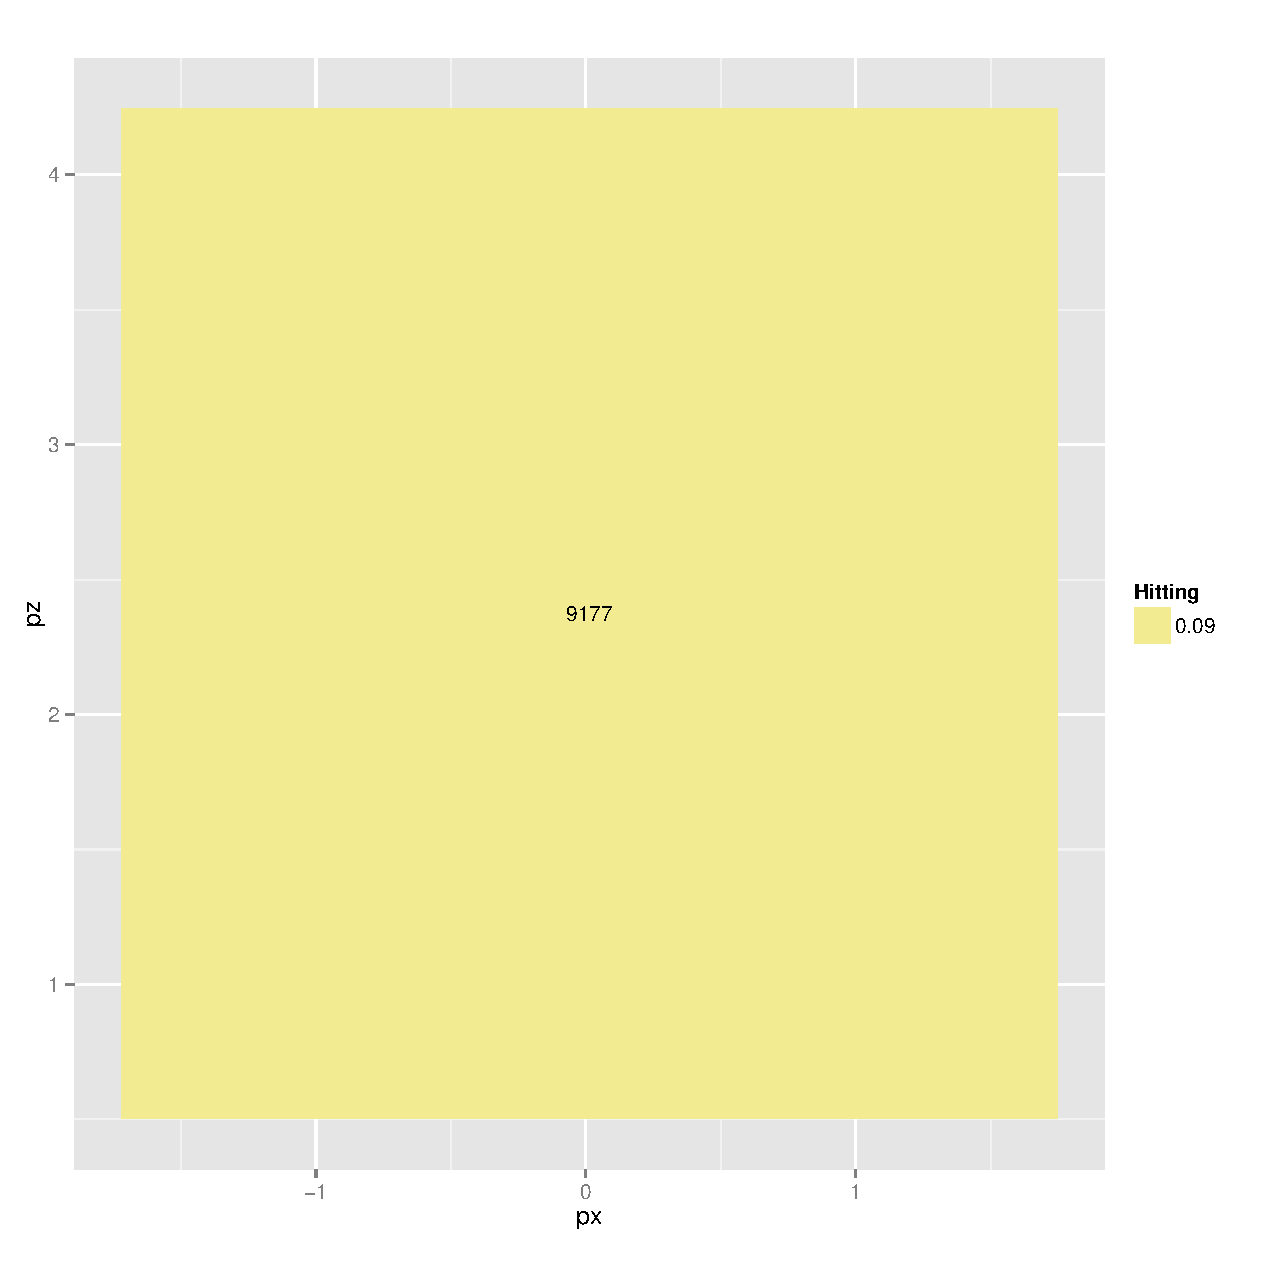
\includegraphics[scale=.2]{Images/Chapter1x1.pdf}
      	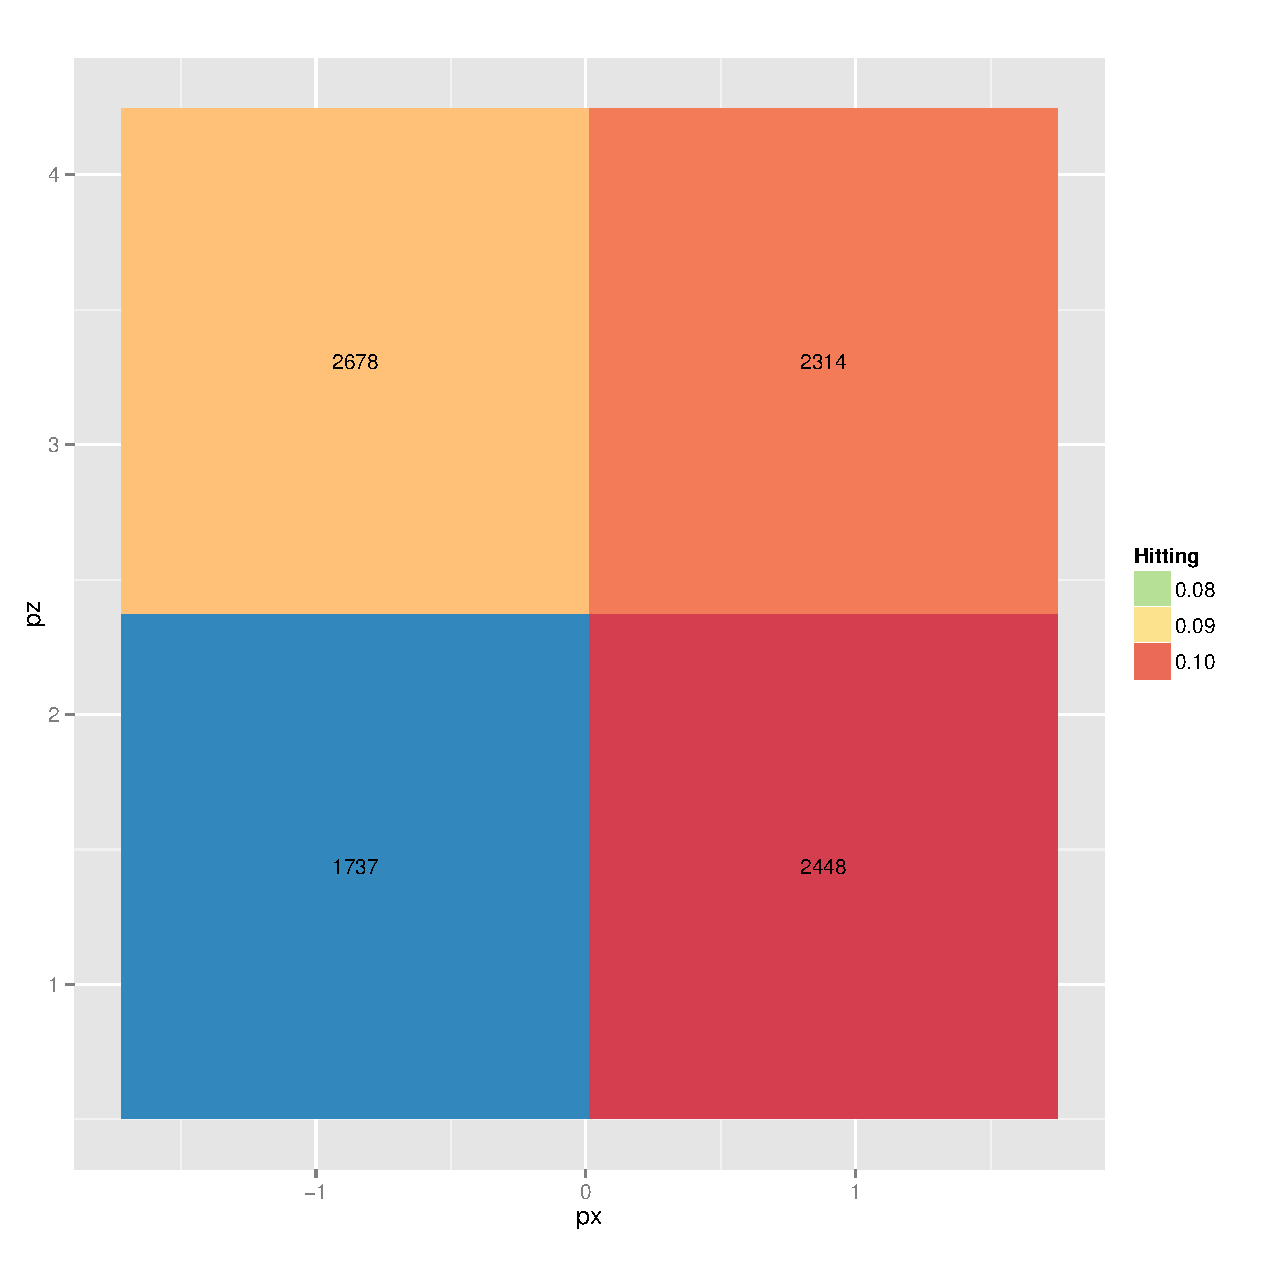
\includegraphics[scale=.2]{Images/Chapter2x2.pdf}
      	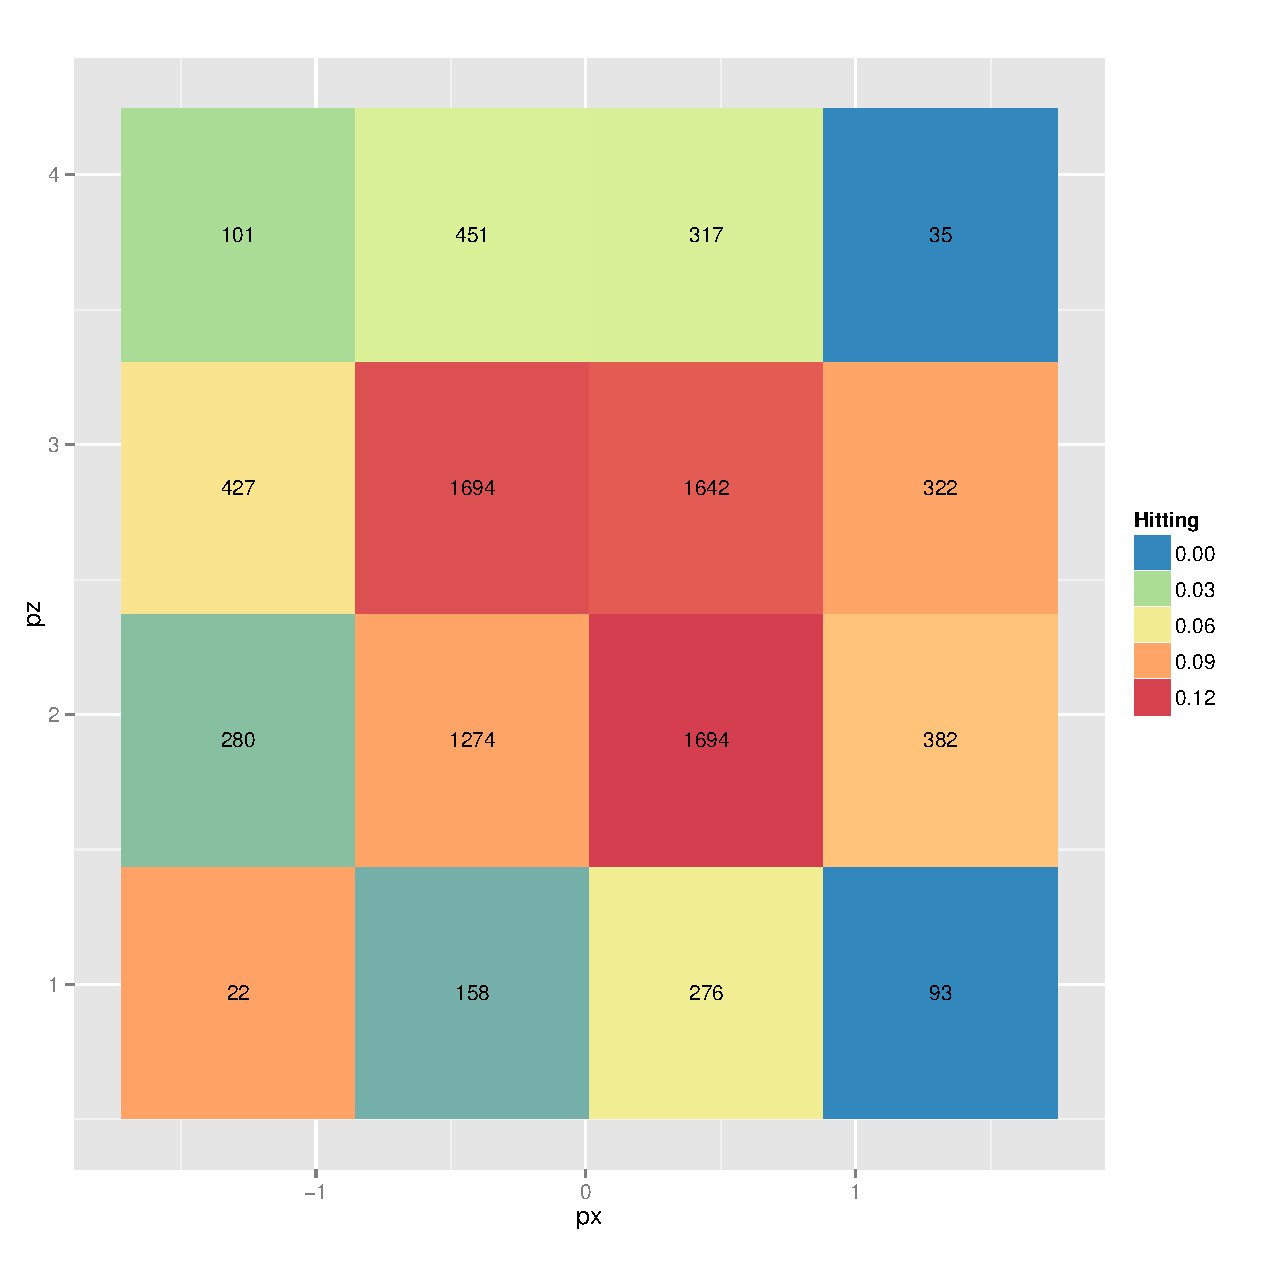
\includegraphics[scale=.2]{Images/Chapter4x4.pdf}
      	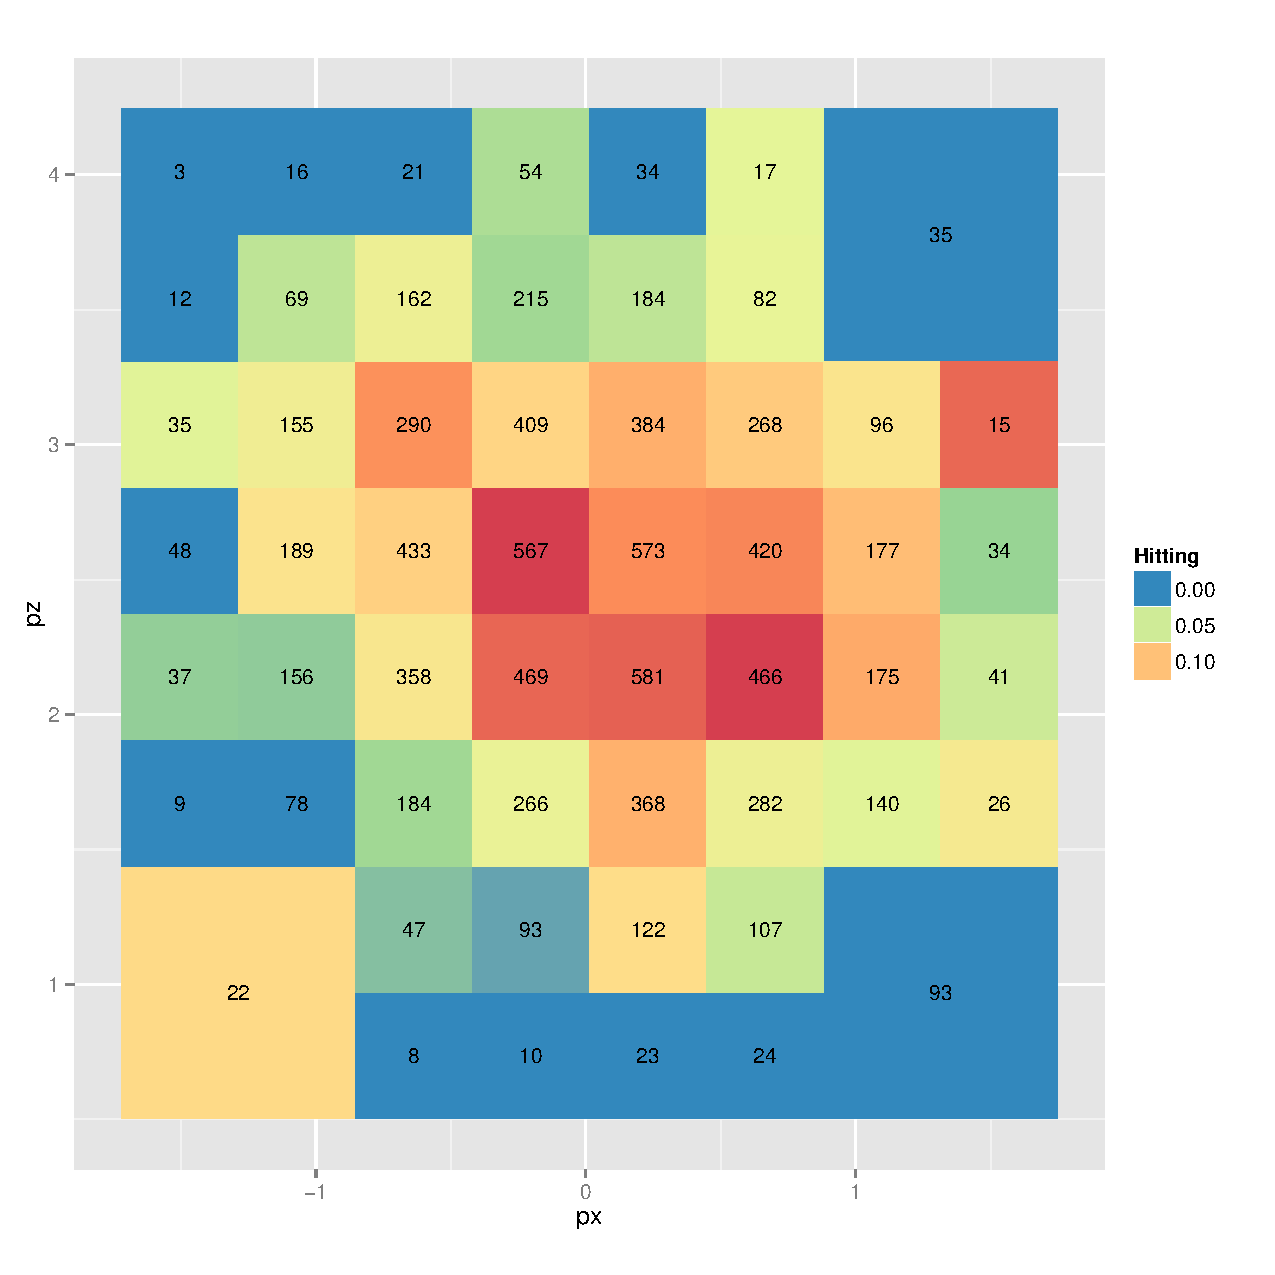
\includegraphics[scale=.2]{Images/Chapter8x8_100.pdf}
      	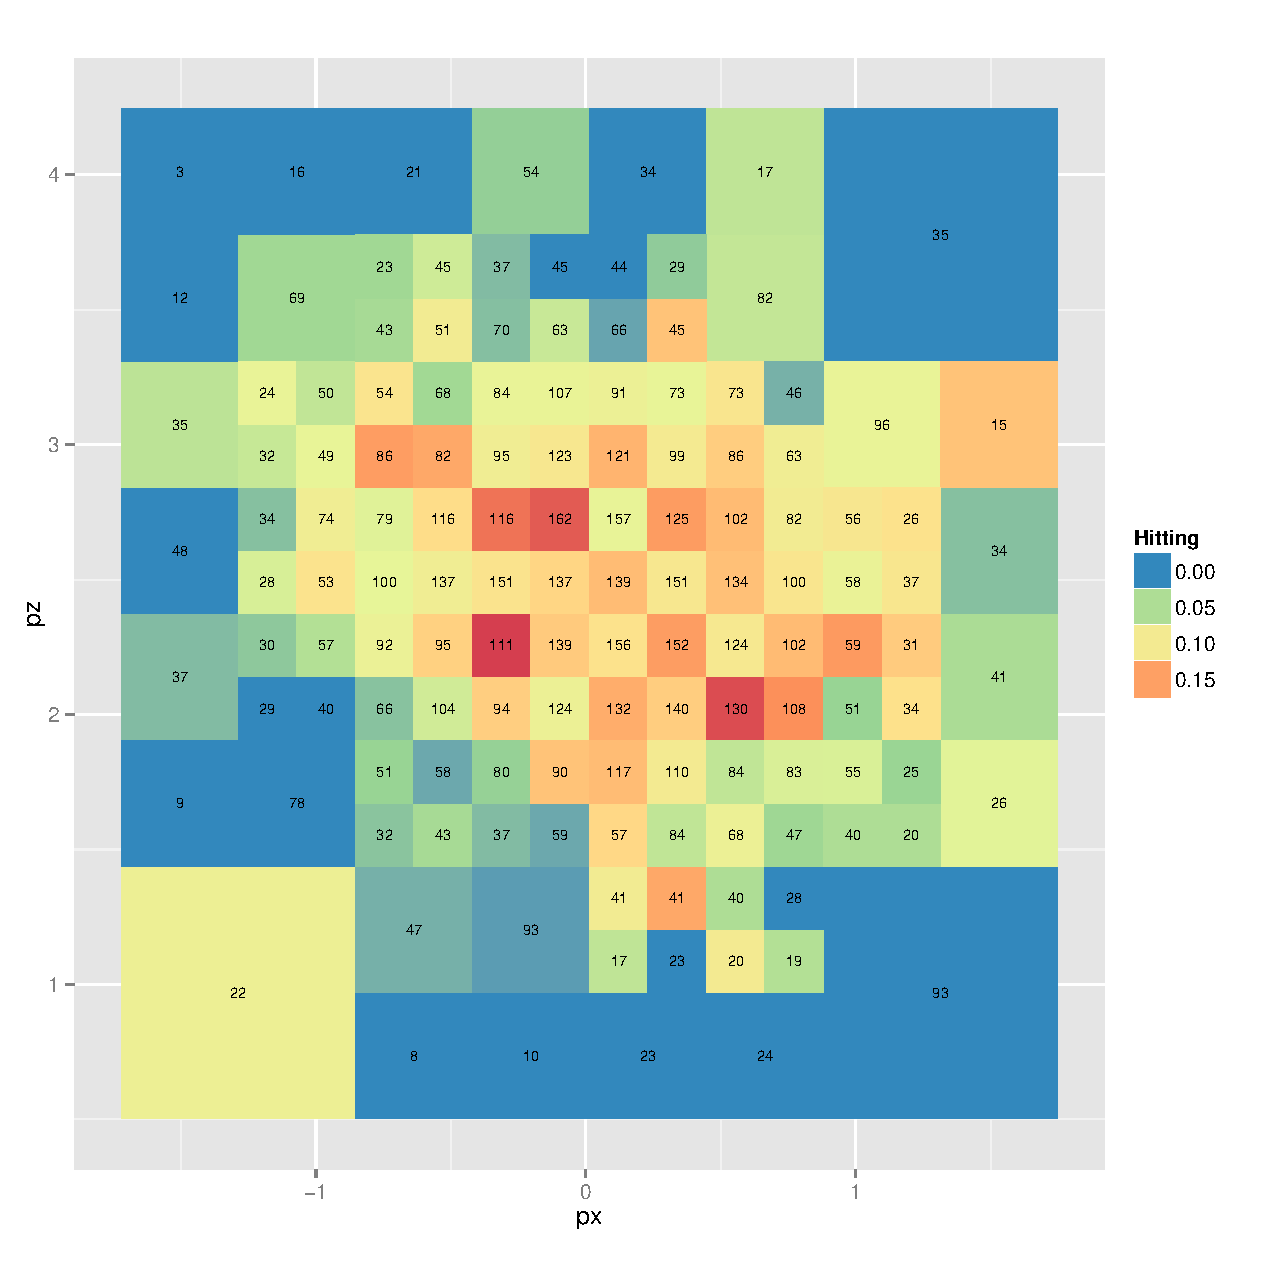
\includegraphics[scale=.2]{Images/Chapter16x16_100.pdf}
      	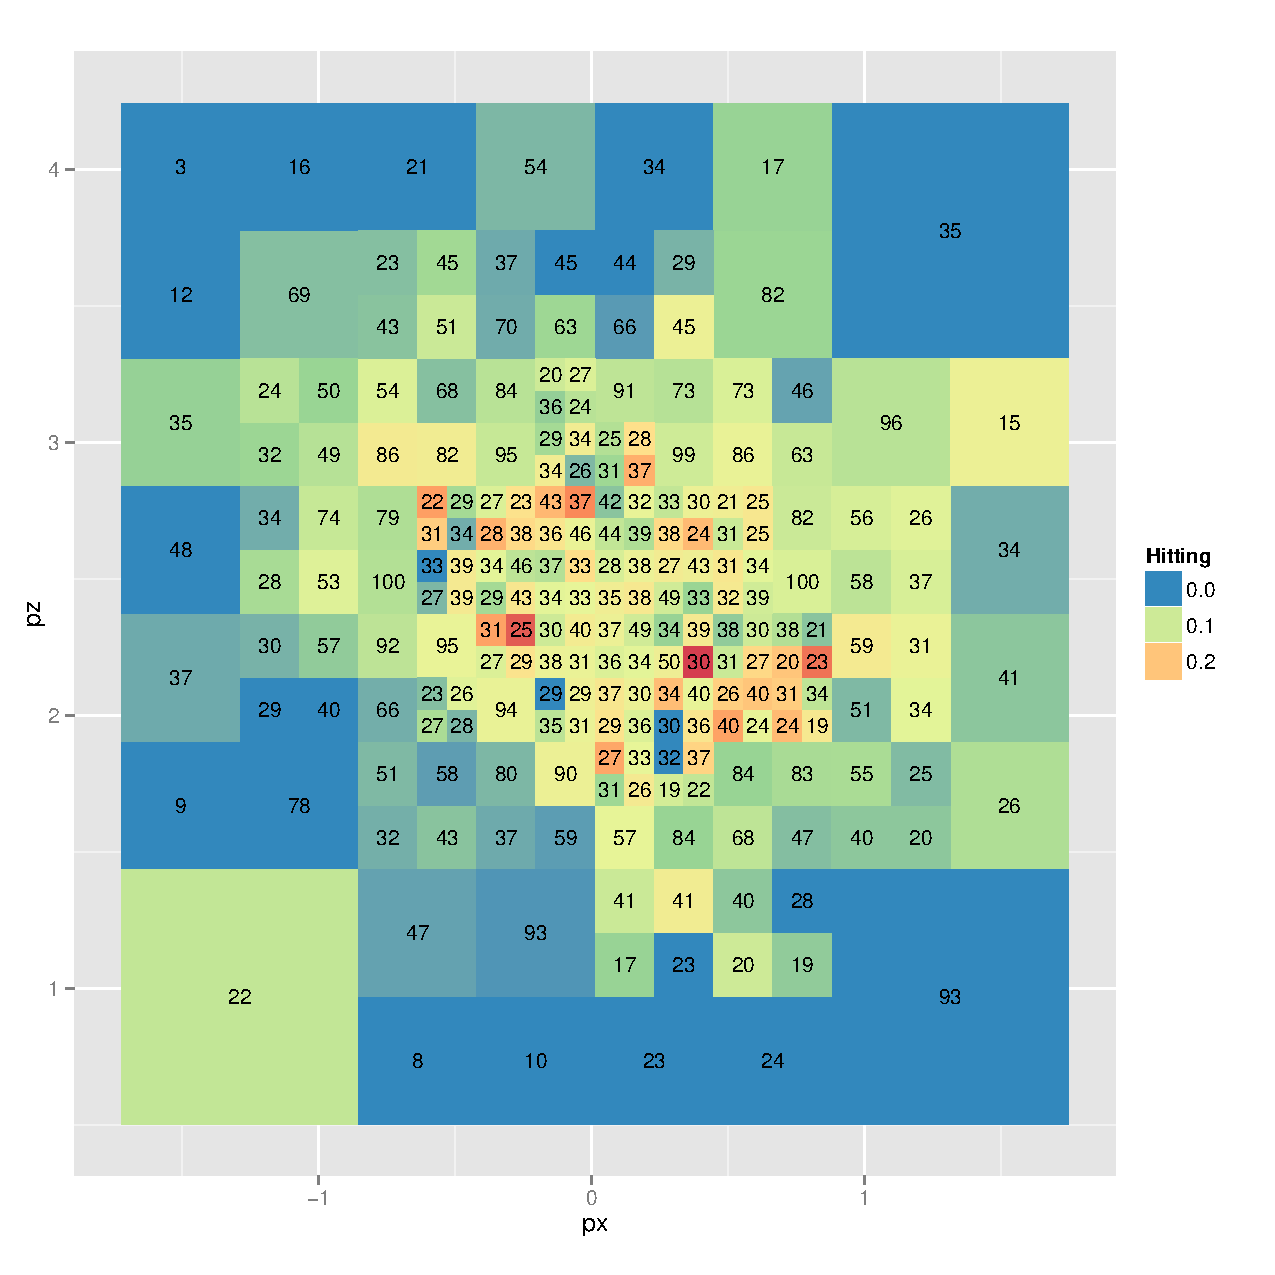
\includegraphics[scale=.2]{Images/Chapter32x32_100.pdf}
      	\caption{These heat maps convey the empirical batting average of batter 425509, Johnny Peralta, in each boxed region of the hitting zone. Each box maps $\hat{p}_{b}$ to a color. The number printed on each box represents the number of pitches the hitter swung at that passed through that box. All boxes with a sample size greater than 100 in each heat map have been subdivided in the subsequent heat map.}
\end{figure} 	
Compare this sequence to Figure 7, where the stopping rule was $n_{b} < 100$. The top row of heat maps in Figure 7 and Figure 8 are identical, but notice in the four by four heat map that $100 < n_{(2,1)} < 200, \text{ and } 100 < n_{(1,4)} < 200$. This implies one stopping rule applies, but the other does not.
        \begin{figure}[H]
      	\centering      
      	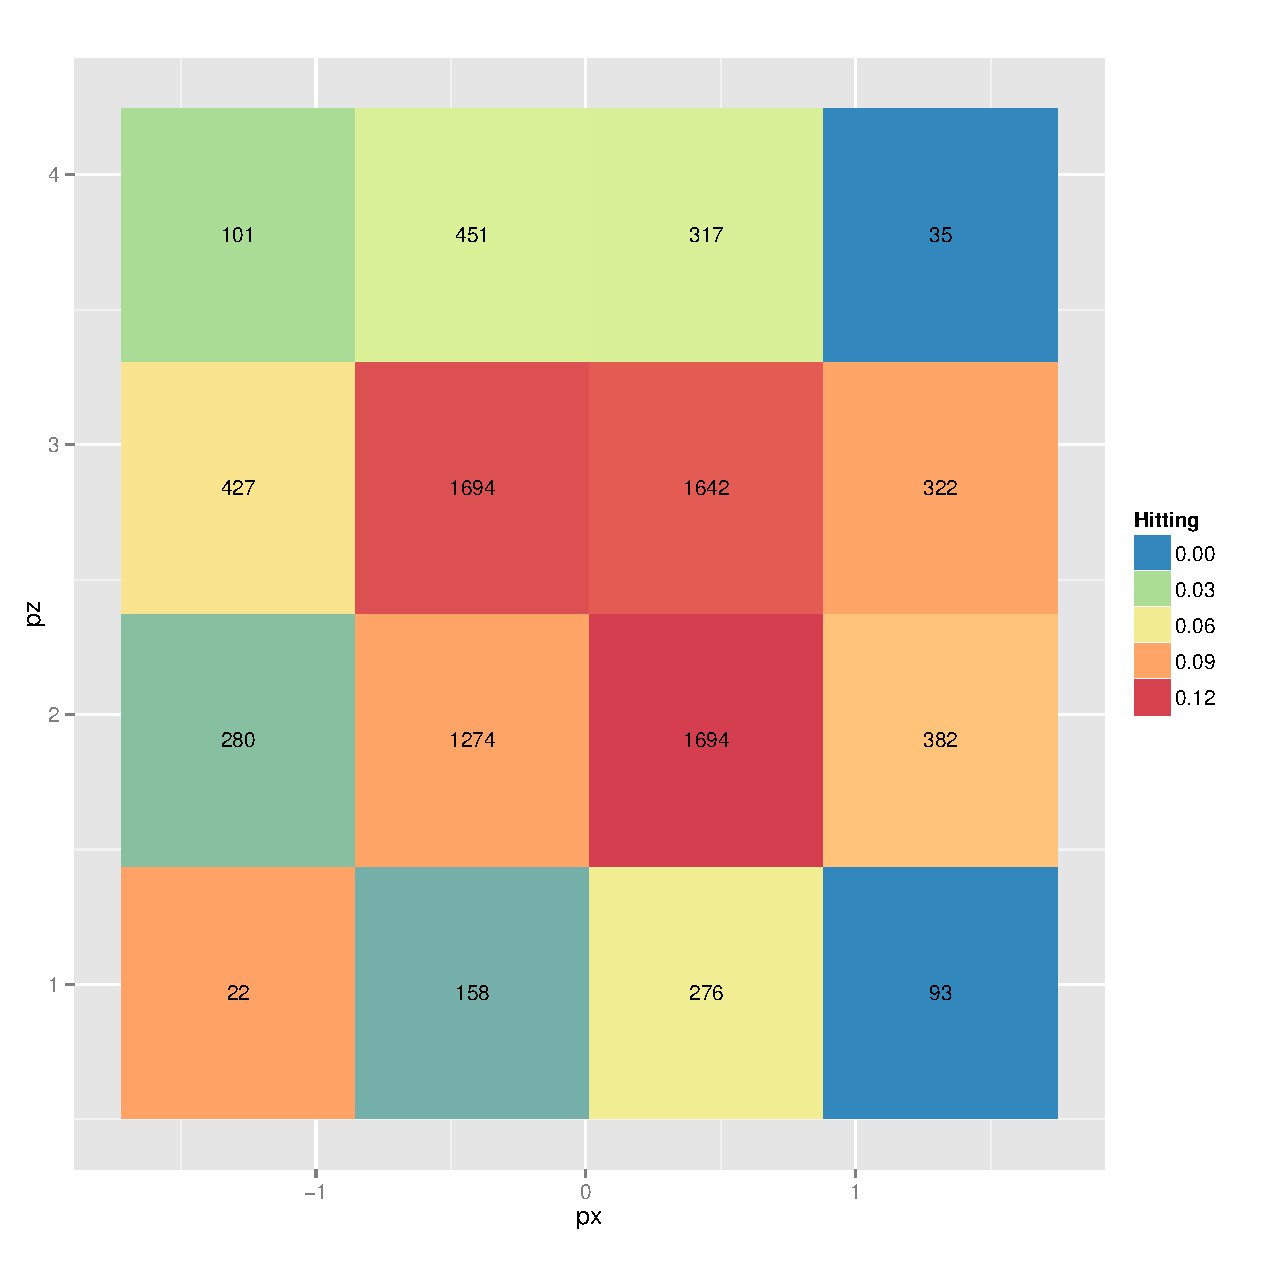
\includegraphics[scale=.2]{Images/Chapter4x4.pdf}
      	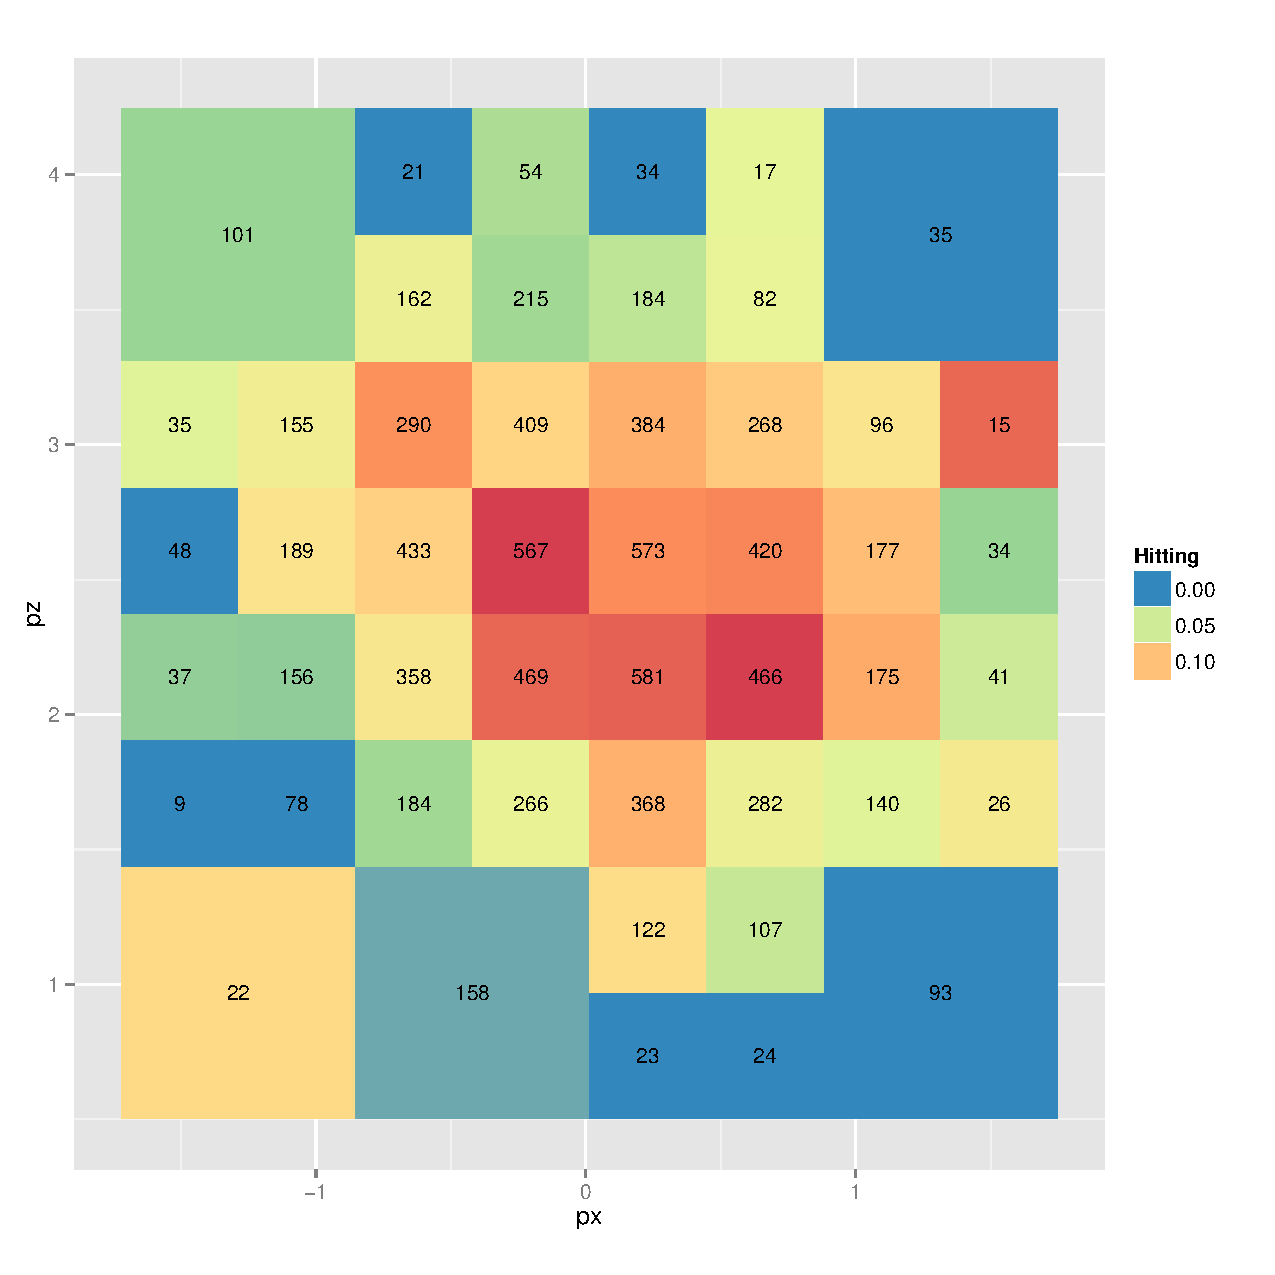
\includegraphics[scale=.2]{Images/Chapter8x8_200.pdf}
      	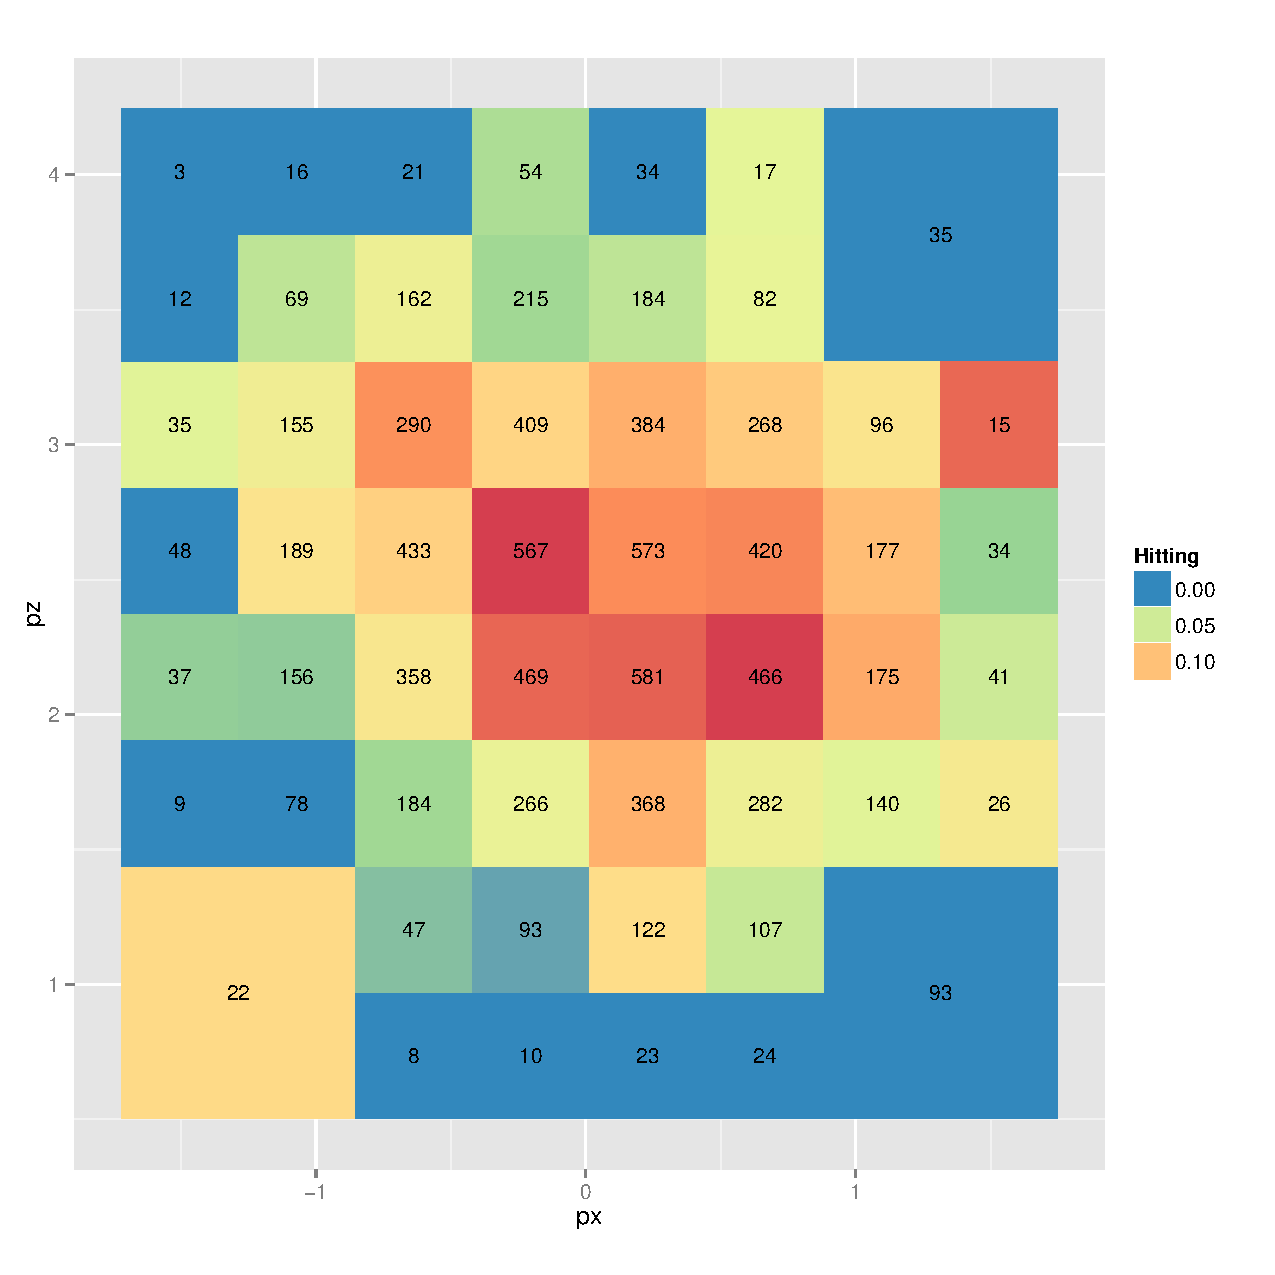
\includegraphics[scale=.2]{Images/Chapter8x8_100.pdf}
      	\caption{...(these images, and others, need labels: (A) (B) (C) etc)}
\end{figure} 
For this reason the bottom left heat maps in Figures 7 and 8, shown in Figure 9, differ in the number of boxes of each size, and the total number of boxes. This divergence continues at the next iteration, where the stopping rule $n_{b} < 100$ requires 28 box subdivisions in Figure 8, map three; and $n_{b} < 200$ gives 16 box subdivisions in Figure 7, map three.

% *Alix: ``I wonder if there's any literature on the physics from a hitter's perspective in terms of how small a difference in location is even detectable.

% *Alix: ``Great start Chris. --> need to add more about how one would now interpret the ``best'' empirical heat map.

\subsection{Appendix: VarResHM, An R Package}


\bibliography{Baseball}

\end{document}